\documentclass[12pt]{article}
\usepackage[utf8]{inputenc}
\usepackage[margin=1.0in]{geometry}
\usepackage[version=4]{mhchem}
\usepackage[separate-uncertainty = true,multi-part-units=single]{siunitx}
\usepackage{amsmath}
\usepackage{amssymb}
\usepackage{graphicx}
\usepackage{xparse}
\usepackage{pgfplots}
\pgfplotsset{compat=1.18}
\usepackage[skip=10pt plus1pt, indent=20pt]{parskip}
\usepackage{booktabs}
%\usepackage{pdflscape}

\usepackage{bibentry}

\NewDocumentCommand{\codeword}{v}{%
\texttt{\textcolor{black}{#1}}%
}

\DeclareSIUnit\gauss{G}
\DeclareSIUnit\erg{erg}
\DeclareSIUnit\year{yr}

\title{\vspace{-2em} {\bf Light Curve Observations of Eclipsing Contact Binaries}}
\author{Matt Ketkaroonkul, Thomas Sweeney, \\ Peter Zhou, Mikhail Mazuzakov}
\date{June 4, 2023}

\DeclareSIUnit\day{d}
\begin{document}

\maketitle

\section{Abstract}
\section{Introduction}

Eclipsing Contact Binaries consist of two stars orbiting each other in close proximity, periodically passing in front of each other, leading to a characteristic variation in their observed brightness over time. Contact Binaries orbit so close to one another that their Roche lobes overlap, allowing the exchange of stellar material. Quantifying light curves for eclipsing binaries is an essential task in the field of astrophysics, enabling the detailed study of these fascinating systems. By accurately measuring and analyzing these light curves, astronomers can derive fundamental parameters of the binary system, such as the stellar masses, radii, and orbital parameters. More importantly, the study of eclipsing contact binaries has greater implications for understanding the general behavior of binary star systems, as well as stellar evolution and structure.

Understanding the behavior of binary star systems through eclipsing binary observations can aid our understanding of stellar structure. Many binary star systems have close orbits, where the constituent stars exchange stellar matter. This presents a unique opportunity to study stellar atmospheres under continual disturbances by the gravitational pulls of the closely-orbiting companion star. The rapid rotation of these stars also suggests interesting magnetic field and stellar wind behaviors present in these binary star systems \cite{2001icbs.book.....H}. Close binary star systems can also influence the stellar evolution of each constituent star. As posited by Yakut and Eggleton (2005), at longer timescales, close binary star systems may evolve such that the masses of the constituent stars equalize. As the stars’ masses substantially change, their stellar evolution path may have drastically changed as well \cite{2005ApJ...629.1055Y}.

	TZ Boo is an eclipsing contact binary system located in the Boötes constellation. Its constituent stars are both G type stars. The other system we observed, CC Com, is located in the Coma Berenices constellation and consists of K type stars. The purpose of our project is to observe light curves for each of the star systems and determine their orbital properties for comparison with previous data and analyses of the eclipsing contact binaries. Given our time constraints with the Apache Point Observatory (APO) ARCSAT, we picked these eclipsing binary systems for their short orbital period of around 0.3 d. TZ Boo has a period of 0.297 d and CC Com has a period of 0.221 d. 

    We begin with describing the setup and circumstances of our observation project, followed by our process in data reduction. We then analyze our results to compare with previous research, including the results from Yakut and Eggleton (2005) \cite{2005ApJ...629.1055Y}. We conclude our paper by pointing out sources of error, which inform goals to be achieved in future work.

\section{Observations and Data}

Observations were taken from APO ARCSAT on the mornings of April 04, 2023 and May 05, 2023. Local weather conditions were (unfortunately) cloudy skies and a relatively high dust count. Allotted observations were also interrupted by a malfunction of one of the ARCSAT components. As a result, we collected 3 data points for CC Com and 4 data points for TZ Boo. Collecting light curve data involves relative photometric measurements, so calibrating measurements to get an absolute flux reading was not necessary for our project– we were only concerned about reducing overexposure. 

Our observations also did not need to account for spectral information, so our project did not depend heavily on filter choice. So, we decided to pick the filter that reduced the amount of overexposed pixels. We originally picked both B and V filters, though we eventually settled on V filters for both observations of TZ Boo and CC Com as we had the best luck with reducing chances of overexposure. Each exposure was 15 seconds long and taken every 30 minutes.

\subsection{Observation Procedure}
For image noise reduction, we took 7 bias frames, 4 dark frames with 900 seconds of exposure, and 3 flats for the V filter. Data reduction steps were carried out in Jupyter notebooks as follows:

\begin{enumerate}
    \item Bias frames were combined using \codeword{ccdproc}, a Python package handling CCD image processing. The combined frame would be used for multiple subsequent steps
    \item Each raw dark frame had its bias subtracted with the combined bias frame. All bias-subtracted frames were then combined.
    \item Each flat frame (for the V filter) had its bias and dark current subtracted using the combined bias and dark frames resulting from steps 1 and 2. The flat frames were combined.
    \item Each raw frame taken as observation data was processed by subtracting the bias and dark current and then dividing the result by the pixel values of the flat frame. 
\end{enumerate}

\subsection{Data Reduction}
We considered a few photometry methods to determine the relative flux from the processed CCD images. These include the built-in photometric flux from the \codeword{DAOStarFinder} function from the \codeword{photutils.detection} package, and the Aperture (AP) and Point Spread Function (PSF) photometry methods from the same \codeword{photutils} package. From the \codeword{photutils.detection} documentation, the flux reading from \codeword{DAOStarFinder} involves the object flux calculated as the peak density in the convolved image divided by the detection threshold. AP photometry involves applying a circular mask region marking where pixels should be counted and included in the AP flux reading. 

A \codeword{CircularAnnulus} variant of the photometric method may also be applied to more finely distinguish between background sky pixels and object pixels. PSF photometry involves modeling more diffuse objects as a certain function to weight pixels before including them in the flux count. 

To reduce the complexity of the model behind determining relative flux values, we picked AP photometry due to a better transparency on how pixels are included in flux counts. While PSF photometry is robust in determining flux counts for diffuse objects, we determined that AP photometry would still be preferable to recording light curve data for pointlike sources of light. As shown in Figures X and Y, both star system images can be captured with a circular aperture.

\begin{figure}[htpb]
    \begin{center}
        % %% Creator: Matplotlib, PGF backend
%%
%% To include the figure in your LaTeX document, write
%%   \input{<filename>.pgf}
%%
%% Make sure the required packages are loaded in your preamble
%%   \usepackage{pgf}
%%
%% Also ensure that all the required font packages are loaded; for instance,
%% the lmodern package is sometimes necessary when using math font.
%%   \usepackage{lmodern}
%%
%% Figures using additional raster images can only be included by \input if
%% they are in the same directory as the main LaTeX file. For loading figures
%% from other directories you can use the `import` package
%%   \usepackage{import}
%%
%% and then include the figures with
%%   \import{<path to file>}{<filename>.pgf}
%%
%% Matplotlib used the following preamble
%%
\begingroup%
\makeatletter%
\begin{pgfpicture}%
\pgfpathrectangle{\pgfpointorigin}{\pgfqpoint{5.000000in}{5.000000in}}%
\pgfusepath{use as bounding box, clip}%
\begin{pgfscope}%
\pgfsetbuttcap%
\pgfsetmiterjoin%
\pgfsetlinewidth{0.000000pt}%
\definecolor{currentstroke}{rgb}{1.000000,1.000000,1.000000}%
\pgfsetstrokecolor{currentstroke}%
\pgfsetstrokeopacity{0.000000}%
\pgfsetdash{}{0pt}%
\pgfpathmoveto{\pgfqpoint{0.000000in}{0.000000in}}%
\pgfpathlineto{\pgfqpoint{5.000000in}{0.000000in}}%
\pgfpathlineto{\pgfqpoint{5.000000in}{5.000000in}}%
\pgfpathlineto{\pgfqpoint{0.000000in}{5.000000in}}%
\pgfpathlineto{\pgfqpoint{0.000000in}{0.000000in}}%
\pgfpathclose%
\pgfusepath{}%
\end{pgfscope}%
\begin{pgfscope}%
\pgfsetbuttcap%
\pgfsetmiterjoin%
\definecolor{currentfill}{rgb}{1.000000,1.000000,1.000000}%
\pgfsetfillcolor{currentfill}%
\pgfsetlinewidth{0.000000pt}%
\definecolor{currentstroke}{rgb}{0.000000,0.000000,0.000000}%
\pgfsetstrokecolor{currentstroke}%
\pgfsetstrokeopacity{0.000000}%
\pgfsetdash{}{0pt}%
\pgfpathmoveto{\pgfqpoint{0.125000in}{0.502998in}}%
\pgfpathlineto{\pgfqpoint{4.334571in}{0.502998in}}%
\pgfpathlineto{\pgfqpoint{4.334571in}{4.712569in}}%
\pgfpathlineto{\pgfqpoint{0.125000in}{4.712569in}}%
\pgfpathlineto{\pgfqpoint{0.125000in}{0.502998in}}%
\pgfpathclose%
\pgfusepath{fill}%
\end{pgfscope}%
\begin{pgfscope}%
\pgfpathrectangle{\pgfqpoint{0.125000in}{0.502998in}}{\pgfqpoint{4.209571in}{4.209571in}}%
\pgfusepath{clip}%
\pgfsys@transformshift{0.125000in}{0.502998in}%
\pgftext[left,bottom]{\includegraphics[interpolate=true,width=4.210000in,height=4.210000in]{cc-com_reduced-example-img0.png}}%
\end{pgfscope}%
\begin{pgfscope}%
\pgfpathrectangle{\pgfqpoint{0.125000in}{0.502998in}}{\pgfqpoint{4.209571in}{4.209571in}}%
\pgfusepath{clip}%
\pgfsetbuttcap%
\pgfsetmiterjoin%
\pgfsetlinewidth{1.003750pt}%
\definecolor{currentstroke}{rgb}{1.000000,0.000000,0.000000}%
\pgfsetstrokecolor{currentstroke}%
\pgfsetstrokeopacity{0.500000}%
\pgfsetdash{}{0pt}%
\pgfpathmoveto{\pgfqpoint{2.229785in}{2.186826in}}%
\pgfpathcurveto{\pgfqpoint{2.341424in}{2.186826in}}{\pgfqpoint{2.448506in}{2.231181in}}{\pgfqpoint{2.527447in}{2.310122in}}%
\pgfpathcurveto{\pgfqpoint{2.606388in}{2.389063in}}{\pgfqpoint{2.650742in}{2.496144in}}{\pgfqpoint{2.650742in}{2.607784in}}%
\pgfpathcurveto{\pgfqpoint{2.650742in}{2.719423in}}{\pgfqpoint{2.606388in}{2.826504in}}{\pgfqpoint{2.527447in}{2.905445in}}%
\pgfpathcurveto{\pgfqpoint{2.448506in}{2.984386in}}{\pgfqpoint{2.341424in}{3.028741in}}{\pgfqpoint{2.229785in}{3.028741in}}%
\pgfpathcurveto{\pgfqpoint{2.118146in}{3.028741in}}{\pgfqpoint{2.011064in}{2.984386in}}{\pgfqpoint{1.932124in}{2.905445in}}%
\pgfpathcurveto{\pgfqpoint{1.853183in}{2.826504in}}{\pgfqpoint{1.808828in}{2.719423in}}{\pgfqpoint{1.808828in}{2.607784in}}%
\pgfpathcurveto{\pgfqpoint{1.808828in}{2.496144in}}{\pgfqpoint{1.853183in}{2.389063in}}{\pgfqpoint{1.932124in}{2.310122in}}%
\pgfpathcurveto{\pgfqpoint{2.011064in}{2.231181in}}{\pgfqpoint{2.118146in}{2.186826in}}{\pgfqpoint{2.229785in}{2.186826in}}%
\pgfpathlineto{\pgfqpoint{2.229785in}{2.186826in}}%
\pgfpathclose%
\pgfusepath{stroke}%
\end{pgfscope}%
\begin{pgfscope}%
\pgfsetbuttcap%
\pgfsetroundjoin%
\definecolor{currentfill}{rgb}{0.000000,0.000000,0.000000}%
\pgfsetfillcolor{currentfill}%
\pgfsetlinewidth{0.803000pt}%
\definecolor{currentstroke}{rgb}{0.000000,0.000000,0.000000}%
\pgfsetstrokecolor{currentstroke}%
\pgfsetdash{}{0pt}%
\pgfsys@defobject{currentmarker}{\pgfqpoint{0.000000in}{-0.048611in}}{\pgfqpoint{0.000000in}{0.000000in}}{%
\pgfpathmoveto{\pgfqpoint{0.000000in}{0.000000in}}%
\pgfpathlineto{\pgfqpoint{0.000000in}{-0.048611in}}%
\pgfusepath{stroke,fill}%
}%
\begin{pgfscope}%
\pgfsys@transformshift{0.125000in}{0.502998in}%
\pgfsys@useobject{currentmarker}{}%
\end{pgfscope}%
\end{pgfscope}%
\begin{pgfscope}%
\definecolor{textcolor}{rgb}{0.000000,0.000000,0.000000}%
\pgfsetstrokecolor{textcolor}%
\pgfsetfillcolor{textcolor}%
\pgftext[x=0.125000in,y=0.405776in,,top]{\color{textcolor}\rmfamily\fontsize{10.000000}{12.000000}\selectfont \(\displaystyle {0}\)}%
\end{pgfscope}%
\begin{pgfscope}%
\pgfsetbuttcap%
\pgfsetroundjoin%
\definecolor{currentfill}{rgb}{0.000000,0.000000,0.000000}%
\pgfsetfillcolor{currentfill}%
\pgfsetlinewidth{0.803000pt}%
\definecolor{currentstroke}{rgb}{0.000000,0.000000,0.000000}%
\pgfsetstrokecolor{currentstroke}%
\pgfsetdash{}{0pt}%
\pgfsys@defobject{currentmarker}{\pgfqpoint{0.000000in}{-0.048611in}}{\pgfqpoint{0.000000in}{0.000000in}}{%
\pgfpathmoveto{\pgfqpoint{0.000000in}{0.000000in}}%
\pgfpathlineto{\pgfqpoint{0.000000in}{-0.048611in}}%
\pgfusepath{stroke,fill}%
}%
\begin{pgfscope}%
\pgfsys@transformshift{0.966914in}{0.502998in}%
\pgfsys@useobject{currentmarker}{}%
\end{pgfscope}%
\end{pgfscope}%
\begin{pgfscope}%
\definecolor{textcolor}{rgb}{0.000000,0.000000,0.000000}%
\pgfsetstrokecolor{textcolor}%
\pgfsetfillcolor{textcolor}%
\pgftext[x=0.966914in,y=0.405776in,,top]{\color{textcolor}\rmfamily\fontsize{10.000000}{12.000000}\selectfont \(\displaystyle {20}\)}%
\end{pgfscope}%
\begin{pgfscope}%
\pgfsetbuttcap%
\pgfsetroundjoin%
\definecolor{currentfill}{rgb}{0.000000,0.000000,0.000000}%
\pgfsetfillcolor{currentfill}%
\pgfsetlinewidth{0.803000pt}%
\definecolor{currentstroke}{rgb}{0.000000,0.000000,0.000000}%
\pgfsetstrokecolor{currentstroke}%
\pgfsetdash{}{0pt}%
\pgfsys@defobject{currentmarker}{\pgfqpoint{0.000000in}{-0.048611in}}{\pgfqpoint{0.000000in}{0.000000in}}{%
\pgfpathmoveto{\pgfqpoint{0.000000in}{0.000000in}}%
\pgfpathlineto{\pgfqpoint{0.000000in}{-0.048611in}}%
\pgfusepath{stroke,fill}%
}%
\begin{pgfscope}%
\pgfsys@transformshift{1.808828in}{0.502998in}%
\pgfsys@useobject{currentmarker}{}%
\end{pgfscope}%
\end{pgfscope}%
\begin{pgfscope}%
\definecolor{textcolor}{rgb}{0.000000,0.000000,0.000000}%
\pgfsetstrokecolor{textcolor}%
\pgfsetfillcolor{textcolor}%
\pgftext[x=1.808828in,y=0.405776in,,top]{\color{textcolor}\rmfamily\fontsize{10.000000}{12.000000}\selectfont \(\displaystyle {40}\)}%
\end{pgfscope}%
\begin{pgfscope}%
\pgfsetbuttcap%
\pgfsetroundjoin%
\definecolor{currentfill}{rgb}{0.000000,0.000000,0.000000}%
\pgfsetfillcolor{currentfill}%
\pgfsetlinewidth{0.803000pt}%
\definecolor{currentstroke}{rgb}{0.000000,0.000000,0.000000}%
\pgfsetstrokecolor{currentstroke}%
\pgfsetdash{}{0pt}%
\pgfsys@defobject{currentmarker}{\pgfqpoint{0.000000in}{-0.048611in}}{\pgfqpoint{0.000000in}{0.000000in}}{%
\pgfpathmoveto{\pgfqpoint{0.000000in}{0.000000in}}%
\pgfpathlineto{\pgfqpoint{0.000000in}{-0.048611in}}%
\pgfusepath{stroke,fill}%
}%
\begin{pgfscope}%
\pgfsys@transformshift{2.650742in}{0.502998in}%
\pgfsys@useobject{currentmarker}{}%
\end{pgfscope}%
\end{pgfscope}%
\begin{pgfscope}%
\definecolor{textcolor}{rgb}{0.000000,0.000000,0.000000}%
\pgfsetstrokecolor{textcolor}%
\pgfsetfillcolor{textcolor}%
\pgftext[x=2.650742in,y=0.405776in,,top]{\color{textcolor}\rmfamily\fontsize{10.000000}{12.000000}\selectfont \(\displaystyle {60}\)}%
\end{pgfscope}%
\begin{pgfscope}%
\pgfsetbuttcap%
\pgfsetroundjoin%
\definecolor{currentfill}{rgb}{0.000000,0.000000,0.000000}%
\pgfsetfillcolor{currentfill}%
\pgfsetlinewidth{0.803000pt}%
\definecolor{currentstroke}{rgb}{0.000000,0.000000,0.000000}%
\pgfsetstrokecolor{currentstroke}%
\pgfsetdash{}{0pt}%
\pgfsys@defobject{currentmarker}{\pgfqpoint{0.000000in}{-0.048611in}}{\pgfqpoint{0.000000in}{0.000000in}}{%
\pgfpathmoveto{\pgfqpoint{0.000000in}{0.000000in}}%
\pgfpathlineto{\pgfqpoint{0.000000in}{-0.048611in}}%
\pgfusepath{stroke,fill}%
}%
\begin{pgfscope}%
\pgfsys@transformshift{3.492656in}{0.502998in}%
\pgfsys@useobject{currentmarker}{}%
\end{pgfscope}%
\end{pgfscope}%
\begin{pgfscope}%
\definecolor{textcolor}{rgb}{0.000000,0.000000,0.000000}%
\pgfsetstrokecolor{textcolor}%
\pgfsetfillcolor{textcolor}%
\pgftext[x=3.492656in,y=0.405776in,,top]{\color{textcolor}\rmfamily\fontsize{10.000000}{12.000000}\selectfont \(\displaystyle {80}\)}%
\end{pgfscope}%
\begin{pgfscope}%
\pgfsetbuttcap%
\pgfsetroundjoin%
\definecolor{currentfill}{rgb}{0.000000,0.000000,0.000000}%
\pgfsetfillcolor{currentfill}%
\pgfsetlinewidth{0.803000pt}%
\definecolor{currentstroke}{rgb}{0.000000,0.000000,0.000000}%
\pgfsetstrokecolor{currentstroke}%
\pgfsetdash{}{0pt}%
\pgfsys@defobject{currentmarker}{\pgfqpoint{0.000000in}{-0.048611in}}{\pgfqpoint{0.000000in}{0.000000in}}{%
\pgfpathmoveto{\pgfqpoint{0.000000in}{0.000000in}}%
\pgfpathlineto{\pgfqpoint{0.000000in}{-0.048611in}}%
\pgfusepath{stroke,fill}%
}%
\begin{pgfscope}%
\pgfsys@transformshift{4.334571in}{0.502998in}%
\pgfsys@useobject{currentmarker}{}%
\end{pgfscope}%
\end{pgfscope}%
\begin{pgfscope}%
\definecolor{textcolor}{rgb}{0.000000,0.000000,0.000000}%
\pgfsetstrokecolor{textcolor}%
\pgfsetfillcolor{textcolor}%
\pgftext[x=4.334571in,y=0.405776in,,top]{\color{textcolor}\rmfamily\fontsize{10.000000}{12.000000}\selectfont \(\displaystyle {100}\)}%
\end{pgfscope}%
\begin{pgfscope}%
\definecolor{textcolor}{rgb}{0.000000,0.000000,0.000000}%
\pgfsetstrokecolor{textcolor}%
\pgfsetfillcolor{textcolor}%
\pgftext[x=2.229785in,y=0.226764in,,top]{\color{textcolor}\rmfamily\fontsize{10.000000}{12.000000}\selectfont x Position}%
\end{pgfscope}%
\begin{pgfscope}%
\pgfsetbuttcap%
\pgfsetroundjoin%
\definecolor{currentfill}{rgb}{0.000000,0.000000,0.000000}%
\pgfsetfillcolor{currentfill}%
\pgfsetlinewidth{0.803000pt}%
\definecolor{currentstroke}{rgb}{0.000000,0.000000,0.000000}%
\pgfsetstrokecolor{currentstroke}%
\pgfsetdash{}{0pt}%
\pgfsys@defobject{currentmarker}{\pgfqpoint{-0.048611in}{0.000000in}}{\pgfqpoint{-0.000000in}{0.000000in}}{%
\pgfpathmoveto{\pgfqpoint{-0.000000in}{0.000000in}}%
\pgfpathlineto{\pgfqpoint{-0.048611in}{0.000000in}}%
\pgfusepath{stroke,fill}%
}%
\begin{pgfscope}%
\pgfsys@transformshift{0.125000in}{0.502998in}%
\pgfsys@useobject{currentmarker}{}%
\end{pgfscope}%
\end{pgfscope}%
\begin{pgfscope}%
\definecolor{textcolor}{rgb}{0.000000,0.000000,0.000000}%
\pgfsetstrokecolor{textcolor}%
\pgfsetfillcolor{textcolor}%
\pgftext[x=-0.041667in, y=0.454773in, left, base]{\color{textcolor}\rmfamily\fontsize{10.000000}{12.000000}\selectfont \(\displaystyle {0}\)}%
\end{pgfscope}%
\begin{pgfscope}%
\pgfsetbuttcap%
\pgfsetroundjoin%
\definecolor{currentfill}{rgb}{0.000000,0.000000,0.000000}%
\pgfsetfillcolor{currentfill}%
\pgfsetlinewidth{0.803000pt}%
\definecolor{currentstroke}{rgb}{0.000000,0.000000,0.000000}%
\pgfsetstrokecolor{currentstroke}%
\pgfsetdash{}{0pt}%
\pgfsys@defobject{currentmarker}{\pgfqpoint{-0.048611in}{0.000000in}}{\pgfqpoint{-0.000000in}{0.000000in}}{%
\pgfpathmoveto{\pgfqpoint{-0.000000in}{0.000000in}}%
\pgfpathlineto{\pgfqpoint{-0.048611in}{0.000000in}}%
\pgfusepath{stroke,fill}%
}%
\begin{pgfscope}%
\pgfsys@transformshift{0.125000in}{1.344912in}%
\pgfsys@useobject{currentmarker}{}%
\end{pgfscope}%
\end{pgfscope}%
\begin{pgfscope}%
\definecolor{textcolor}{rgb}{0.000000,0.000000,0.000000}%
\pgfsetstrokecolor{textcolor}%
\pgfsetfillcolor{textcolor}%
\pgftext[x=-0.111112in, y=1.296687in, left, base]{\color{textcolor}\rmfamily\fontsize{10.000000}{12.000000}\selectfont \(\displaystyle {20}\)}%
\end{pgfscope}%
\begin{pgfscope}%
\pgfsetbuttcap%
\pgfsetroundjoin%
\definecolor{currentfill}{rgb}{0.000000,0.000000,0.000000}%
\pgfsetfillcolor{currentfill}%
\pgfsetlinewidth{0.803000pt}%
\definecolor{currentstroke}{rgb}{0.000000,0.000000,0.000000}%
\pgfsetstrokecolor{currentstroke}%
\pgfsetdash{}{0pt}%
\pgfsys@defobject{currentmarker}{\pgfqpoint{-0.048611in}{0.000000in}}{\pgfqpoint{-0.000000in}{0.000000in}}{%
\pgfpathmoveto{\pgfqpoint{-0.000000in}{0.000000in}}%
\pgfpathlineto{\pgfqpoint{-0.048611in}{0.000000in}}%
\pgfusepath{stroke,fill}%
}%
\begin{pgfscope}%
\pgfsys@transformshift{0.125000in}{2.186826in}%
\pgfsys@useobject{currentmarker}{}%
\end{pgfscope}%
\end{pgfscope}%
\begin{pgfscope}%
\definecolor{textcolor}{rgb}{0.000000,0.000000,0.000000}%
\pgfsetstrokecolor{textcolor}%
\pgfsetfillcolor{textcolor}%
\pgftext[x=-0.111112in, y=2.138601in, left, base]{\color{textcolor}\rmfamily\fontsize{10.000000}{12.000000}\selectfont \(\displaystyle {40}\)}%
\end{pgfscope}%
\begin{pgfscope}%
\pgfsetbuttcap%
\pgfsetroundjoin%
\definecolor{currentfill}{rgb}{0.000000,0.000000,0.000000}%
\pgfsetfillcolor{currentfill}%
\pgfsetlinewidth{0.803000pt}%
\definecolor{currentstroke}{rgb}{0.000000,0.000000,0.000000}%
\pgfsetstrokecolor{currentstroke}%
\pgfsetdash{}{0pt}%
\pgfsys@defobject{currentmarker}{\pgfqpoint{-0.048611in}{0.000000in}}{\pgfqpoint{-0.000000in}{0.000000in}}{%
\pgfpathmoveto{\pgfqpoint{-0.000000in}{0.000000in}}%
\pgfpathlineto{\pgfqpoint{-0.048611in}{0.000000in}}%
\pgfusepath{stroke,fill}%
}%
\begin{pgfscope}%
\pgfsys@transformshift{0.125000in}{3.028741in}%
\pgfsys@useobject{currentmarker}{}%
\end{pgfscope}%
\end{pgfscope}%
\begin{pgfscope}%
\definecolor{textcolor}{rgb}{0.000000,0.000000,0.000000}%
\pgfsetstrokecolor{textcolor}%
\pgfsetfillcolor{textcolor}%
\pgftext[x=-0.111112in, y=2.980515in, left, base]{\color{textcolor}\rmfamily\fontsize{10.000000}{12.000000}\selectfont \(\displaystyle {60}\)}%
\end{pgfscope}%
\begin{pgfscope}%
\pgfsetbuttcap%
\pgfsetroundjoin%
\definecolor{currentfill}{rgb}{0.000000,0.000000,0.000000}%
\pgfsetfillcolor{currentfill}%
\pgfsetlinewidth{0.803000pt}%
\definecolor{currentstroke}{rgb}{0.000000,0.000000,0.000000}%
\pgfsetstrokecolor{currentstroke}%
\pgfsetdash{}{0pt}%
\pgfsys@defobject{currentmarker}{\pgfqpoint{-0.048611in}{0.000000in}}{\pgfqpoint{-0.000000in}{0.000000in}}{%
\pgfpathmoveto{\pgfqpoint{-0.000000in}{0.000000in}}%
\pgfpathlineto{\pgfqpoint{-0.048611in}{0.000000in}}%
\pgfusepath{stroke,fill}%
}%
\begin{pgfscope}%
\pgfsys@transformshift{0.125000in}{3.870655in}%
\pgfsys@useobject{currentmarker}{}%
\end{pgfscope}%
\end{pgfscope}%
\begin{pgfscope}%
\definecolor{textcolor}{rgb}{0.000000,0.000000,0.000000}%
\pgfsetstrokecolor{textcolor}%
\pgfsetfillcolor{textcolor}%
\pgftext[x=-0.111112in, y=3.822429in, left, base]{\color{textcolor}\rmfamily\fontsize{10.000000}{12.000000}\selectfont \(\displaystyle {80}\)}%
\end{pgfscope}%
\begin{pgfscope}%
\pgfsetbuttcap%
\pgfsetroundjoin%
\definecolor{currentfill}{rgb}{0.000000,0.000000,0.000000}%
\pgfsetfillcolor{currentfill}%
\pgfsetlinewidth{0.803000pt}%
\definecolor{currentstroke}{rgb}{0.000000,0.000000,0.000000}%
\pgfsetstrokecolor{currentstroke}%
\pgfsetdash{}{0pt}%
\pgfsys@defobject{currentmarker}{\pgfqpoint{-0.048611in}{0.000000in}}{\pgfqpoint{-0.000000in}{0.000000in}}{%
\pgfpathmoveto{\pgfqpoint{-0.000000in}{0.000000in}}%
\pgfpathlineto{\pgfqpoint{-0.048611in}{0.000000in}}%
\pgfusepath{stroke,fill}%
}%
\begin{pgfscope}%
\pgfsys@transformshift{0.125000in}{4.712569in}%
\pgfsys@useobject{currentmarker}{}%
\end{pgfscope}%
\end{pgfscope}%
\begin{pgfscope}%
\definecolor{textcolor}{rgb}{0.000000,0.000000,0.000000}%
\pgfsetstrokecolor{textcolor}%
\pgfsetfillcolor{textcolor}%
\pgftext[x=-0.180556in, y=4.664344in, left, base]{\color{textcolor}\rmfamily\fontsize{10.000000}{12.000000}\selectfont \(\displaystyle {100}\)}%
\end{pgfscope}%
\begin{pgfscope}%
\definecolor{textcolor}{rgb}{0.000000,0.000000,0.000000}%
\pgfsetstrokecolor{textcolor}%
\pgfsetfillcolor{textcolor}%
\pgftext[x=-0.236112in,y=2.607784in,,bottom,rotate=90.000000]{\color{textcolor}\rmfamily\fontsize{10.000000}{12.000000}\selectfont y Position}%
\end{pgfscope}%
\begin{pgfscope}%
\pgfsetrectcap%
\pgfsetmiterjoin%
\pgfsetlinewidth{0.803000pt}%
\definecolor{currentstroke}{rgb}{0.000000,0.000000,0.000000}%
\pgfsetstrokecolor{currentstroke}%
\pgfsetdash{}{0pt}%
\pgfpathmoveto{\pgfqpoint{0.125000in}{0.502998in}}%
\pgfpathlineto{\pgfqpoint{0.125000in}{4.712569in}}%
\pgfusepath{stroke}%
\end{pgfscope}%
\begin{pgfscope}%
\pgfsetrectcap%
\pgfsetmiterjoin%
\pgfsetlinewidth{0.803000pt}%
\definecolor{currentstroke}{rgb}{0.000000,0.000000,0.000000}%
\pgfsetstrokecolor{currentstroke}%
\pgfsetdash{}{0pt}%
\pgfpathmoveto{\pgfqpoint{4.334571in}{0.502998in}}%
\pgfpathlineto{\pgfqpoint{4.334571in}{4.712569in}}%
\pgfusepath{stroke}%
\end{pgfscope}%
\begin{pgfscope}%
\pgfsetrectcap%
\pgfsetmiterjoin%
\pgfsetlinewidth{0.803000pt}%
\definecolor{currentstroke}{rgb}{0.000000,0.000000,0.000000}%
\pgfsetstrokecolor{currentstroke}%
\pgfsetdash{}{0pt}%
\pgfpathmoveto{\pgfqpoint{0.125000in}{0.502998in}}%
\pgfpathlineto{\pgfqpoint{4.334571in}{0.502998in}}%
\pgfusepath{stroke}%
\end{pgfscope}%
\begin{pgfscope}%
\pgfsetrectcap%
\pgfsetmiterjoin%
\pgfsetlinewidth{0.803000pt}%
\definecolor{currentstroke}{rgb}{0.000000,0.000000,0.000000}%
\pgfsetstrokecolor{currentstroke}%
\pgfsetdash{}{0pt}%
\pgfpathmoveto{\pgfqpoint{0.125000in}{4.712569in}}%
\pgfpathlineto{\pgfqpoint{4.334571in}{4.712569in}}%
\pgfusepath{stroke}%
\end{pgfscope}%
\begin{pgfscope}%
\definecolor{textcolor}{rgb}{0.000000,0.000000,0.000000}%
\pgfsetstrokecolor{textcolor}%
\pgfsetfillcolor{textcolor}%
\pgftext[x=2.229785in,y=4.795902in,,base]{\color{textcolor}\rmfamily\fontsize{12.000000}{14.400000}\selectfont CC COM taken at 2023-05-05T03:47:49.549}%
\end{pgfscope}%
\begin{pgfscope}%
\pgfsetbuttcap%
\pgfsetmiterjoin%
\definecolor{currentfill}{rgb}{1.000000,1.000000,1.000000}%
\pgfsetfillcolor{currentfill}%
\pgfsetlinewidth{0.000000pt}%
\definecolor{currentstroke}{rgb}{0.000000,0.000000,0.000000}%
\pgfsetstrokecolor{currentstroke}%
\pgfsetstrokeopacity{0.000000}%
\pgfsetdash{}{0pt}%
\pgfpathmoveto{\pgfqpoint{4.518797in}{0.489181in}}%
\pgfpathlineto{\pgfqpoint{4.730657in}{0.489181in}}%
\pgfpathlineto{\pgfqpoint{4.730657in}{4.726386in}}%
\pgfpathlineto{\pgfqpoint{4.518797in}{4.726386in}}%
\pgfpathlineto{\pgfqpoint{4.518797in}{0.489181in}}%
\pgfpathclose%
\pgfusepath{fill}%
\end{pgfscope}%
\begin{pgfscope}%
\pgfpathrectangle{\pgfqpoint{4.518797in}{0.489181in}}{\pgfqpoint{0.211860in}{4.237204in}}%
\pgfusepath{clip}%
\pgfsetbuttcap%
\pgfsetmiterjoin%
\definecolor{currentfill}{rgb}{1.000000,1.000000,1.000000}%
\pgfsetfillcolor{currentfill}%
\pgfsetlinewidth{0.010037pt}%
\definecolor{currentstroke}{rgb}{1.000000,1.000000,1.000000}%
\pgfsetstrokecolor{currentstroke}%
\pgfsetdash{}{0pt}%
\pgfusepath{stroke,fill}%
\end{pgfscope}%
\begin{pgfscope}%
\pgfsys@transformshift{4.520000in}{0.490000in}%
\pgftext[left,bottom]{\includegraphics[interpolate=true,width=0.210000in,height=4.235000in]{cc-com_reduced-example-img1.png}}%
\end{pgfscope}%
\begin{pgfscope}%
\pgfsetbuttcap%
\pgfsetroundjoin%
\definecolor{currentfill}{rgb}{0.000000,0.000000,0.000000}%
\pgfsetfillcolor{currentfill}%
\pgfsetlinewidth{0.803000pt}%
\definecolor{currentstroke}{rgb}{0.000000,0.000000,0.000000}%
\pgfsetstrokecolor{currentstroke}%
\pgfsetdash{}{0pt}%
\pgfsys@defobject{currentmarker}{\pgfqpoint{0.000000in}{0.000000in}}{\pgfqpoint{0.048611in}{0.000000in}}{%
\pgfpathmoveto{\pgfqpoint{0.000000in}{0.000000in}}%
\pgfpathlineto{\pgfqpoint{0.048611in}{0.000000in}}%
\pgfusepath{stroke,fill}%
}%
\begin{pgfscope}%
\pgfsys@transformshift{4.730657in}{0.489181in}%
\pgfsys@useobject{currentmarker}{}%
\end{pgfscope}%
\end{pgfscope}%
\begin{pgfscope}%
\definecolor{textcolor}{rgb}{0.000000,0.000000,0.000000}%
\pgfsetstrokecolor{textcolor}%
\pgfsetfillcolor{textcolor}%
\pgftext[x=4.827879in, y=0.440956in, left, base]{\color{textcolor}\rmfamily\fontsize{10.000000}{12.000000}\selectfont \(\displaystyle {30}\)}%
\end{pgfscope}%
\begin{pgfscope}%
\pgfsetbuttcap%
\pgfsetroundjoin%
\definecolor{currentfill}{rgb}{0.000000,0.000000,0.000000}%
\pgfsetfillcolor{currentfill}%
\pgfsetlinewidth{0.803000pt}%
\definecolor{currentstroke}{rgb}{0.000000,0.000000,0.000000}%
\pgfsetstrokecolor{currentstroke}%
\pgfsetdash{}{0pt}%
\pgfsys@defobject{currentmarker}{\pgfqpoint{0.000000in}{0.000000in}}{\pgfqpoint{0.048611in}{0.000000in}}{%
\pgfpathmoveto{\pgfqpoint{0.000000in}{0.000000in}}%
\pgfpathlineto{\pgfqpoint{0.048611in}{0.000000in}}%
\pgfusepath{stroke,fill}%
}%
\begin{pgfscope}%
\pgfsys@transformshift{4.730657in}{1.197015in}%
\pgfsys@useobject{currentmarker}{}%
\end{pgfscope}%
\end{pgfscope}%
\begin{pgfscope}%
\definecolor{textcolor}{rgb}{0.000000,0.000000,0.000000}%
\pgfsetstrokecolor{textcolor}%
\pgfsetfillcolor{textcolor}%
\pgftext[x=4.827879in, y=1.148790in, left, base]{\color{textcolor}\rmfamily\fontsize{10.000000}{12.000000}\selectfont \(\displaystyle {40}\)}%
\end{pgfscope}%
\begin{pgfscope}%
\pgfsetbuttcap%
\pgfsetroundjoin%
\definecolor{currentfill}{rgb}{0.000000,0.000000,0.000000}%
\pgfsetfillcolor{currentfill}%
\pgfsetlinewidth{0.803000pt}%
\definecolor{currentstroke}{rgb}{0.000000,0.000000,0.000000}%
\pgfsetstrokecolor{currentstroke}%
\pgfsetdash{}{0pt}%
\pgfsys@defobject{currentmarker}{\pgfqpoint{0.000000in}{0.000000in}}{\pgfqpoint{0.048611in}{0.000000in}}{%
\pgfpathmoveto{\pgfqpoint{0.000000in}{0.000000in}}%
\pgfpathlineto{\pgfqpoint{0.048611in}{0.000000in}}%
\pgfusepath{stroke,fill}%
}%
\begin{pgfscope}%
\pgfsys@transformshift{4.730657in}{1.975402in}%
\pgfsys@useobject{currentmarker}{}%
\end{pgfscope}%
\end{pgfscope}%
\begin{pgfscope}%
\definecolor{textcolor}{rgb}{0.000000,0.000000,0.000000}%
\pgfsetstrokecolor{textcolor}%
\pgfsetfillcolor{textcolor}%
\pgftext[x=4.827879in, y=1.927177in, left, base]{\color{textcolor}\rmfamily\fontsize{10.000000}{12.000000}\selectfont \(\displaystyle {50}\)}%
\end{pgfscope}%
\begin{pgfscope}%
\pgfsetbuttcap%
\pgfsetroundjoin%
\definecolor{currentfill}{rgb}{0.000000,0.000000,0.000000}%
\pgfsetfillcolor{currentfill}%
\pgfsetlinewidth{0.803000pt}%
\definecolor{currentstroke}{rgb}{0.000000,0.000000,0.000000}%
\pgfsetstrokecolor{currentstroke}%
\pgfsetdash{}{0pt}%
\pgfsys@defobject{currentmarker}{\pgfqpoint{0.000000in}{0.000000in}}{\pgfqpoint{0.048611in}{0.000000in}}{%
\pgfpathmoveto{\pgfqpoint{0.000000in}{0.000000in}}%
\pgfpathlineto{\pgfqpoint{0.048611in}{0.000000in}}%
\pgfusepath{stroke,fill}%
}%
\begin{pgfscope}%
\pgfsys@transformshift{4.730657in}{2.753789in}%
\pgfsys@useobject{currentmarker}{}%
\end{pgfscope}%
\end{pgfscope}%
\begin{pgfscope}%
\definecolor{textcolor}{rgb}{0.000000,0.000000,0.000000}%
\pgfsetstrokecolor{textcolor}%
\pgfsetfillcolor{textcolor}%
\pgftext[x=4.827879in, y=2.705564in, left, base]{\color{textcolor}\rmfamily\fontsize{10.000000}{12.000000}\selectfont \(\displaystyle {60}\)}%
\end{pgfscope}%
\begin{pgfscope}%
\pgfsetbuttcap%
\pgfsetroundjoin%
\definecolor{currentfill}{rgb}{0.000000,0.000000,0.000000}%
\pgfsetfillcolor{currentfill}%
\pgfsetlinewidth{0.803000pt}%
\definecolor{currentstroke}{rgb}{0.000000,0.000000,0.000000}%
\pgfsetstrokecolor{currentstroke}%
\pgfsetdash{}{0pt}%
\pgfsys@defobject{currentmarker}{\pgfqpoint{0.000000in}{0.000000in}}{\pgfqpoint{0.048611in}{0.000000in}}{%
\pgfpathmoveto{\pgfqpoint{0.000000in}{0.000000in}}%
\pgfpathlineto{\pgfqpoint{0.048611in}{0.000000in}}%
\pgfusepath{stroke,fill}%
}%
\begin{pgfscope}%
\pgfsys@transformshift{4.730657in}{3.532176in}%
\pgfsys@useobject{currentmarker}{}%
\end{pgfscope}%
\end{pgfscope}%
\begin{pgfscope}%
\definecolor{textcolor}{rgb}{0.000000,0.000000,0.000000}%
\pgfsetstrokecolor{textcolor}%
\pgfsetfillcolor{textcolor}%
\pgftext[x=4.827879in, y=3.483951in, left, base]{\color{textcolor}\rmfamily\fontsize{10.000000}{12.000000}\selectfont \(\displaystyle {70}\)}%
\end{pgfscope}%
\begin{pgfscope}%
\pgfsetbuttcap%
\pgfsetroundjoin%
\definecolor{currentfill}{rgb}{0.000000,0.000000,0.000000}%
\pgfsetfillcolor{currentfill}%
\pgfsetlinewidth{0.803000pt}%
\definecolor{currentstroke}{rgb}{0.000000,0.000000,0.000000}%
\pgfsetstrokecolor{currentstroke}%
\pgfsetdash{}{0pt}%
\pgfsys@defobject{currentmarker}{\pgfqpoint{0.000000in}{0.000000in}}{\pgfqpoint{0.048611in}{0.000000in}}{%
\pgfpathmoveto{\pgfqpoint{0.000000in}{0.000000in}}%
\pgfpathlineto{\pgfqpoint{0.048611in}{0.000000in}}%
\pgfusepath{stroke,fill}%
}%
\begin{pgfscope}%
\pgfsys@transformshift{4.730657in}{4.310563in}%
\pgfsys@useobject{currentmarker}{}%
\end{pgfscope}%
\end{pgfscope}%
\begin{pgfscope}%
\definecolor{textcolor}{rgb}{0.000000,0.000000,0.000000}%
\pgfsetstrokecolor{textcolor}%
\pgfsetfillcolor{textcolor}%
\pgftext[x=4.827879in, y=4.262338in, left, base]{\color{textcolor}\rmfamily\fontsize{10.000000}{12.000000}\selectfont \(\displaystyle {80}\)}%
\end{pgfscope}%
\begin{pgfscope}%
\pgfsetbuttcap%
\pgfsetroundjoin%
\definecolor{currentfill}{rgb}{0.000000,0.000000,0.000000}%
\pgfsetfillcolor{currentfill}%
\pgfsetlinewidth{0.803000pt}%
\definecolor{currentstroke}{rgb}{0.000000,0.000000,0.000000}%
\pgfsetstrokecolor{currentstroke}%
\pgfsetdash{}{0pt}%
\pgfsys@defobject{currentmarker}{\pgfqpoint{0.000000in}{0.000000in}}{\pgfqpoint{0.048611in}{0.000000in}}{%
\pgfpathmoveto{\pgfqpoint{0.000000in}{0.000000in}}%
\pgfpathlineto{\pgfqpoint{0.048611in}{0.000000in}}%
\pgfusepath{stroke,fill}%
}%
\begin{pgfscope}%
\pgfsys@transformshift{4.730657in}{4.726386in}%
\pgfsys@useobject{currentmarker}{}%
\end{pgfscope}%
\end{pgfscope}%
\begin{pgfscope}%
\definecolor{textcolor}{rgb}{0.000000,0.000000,0.000000}%
\pgfsetstrokecolor{textcolor}%
\pgfsetfillcolor{textcolor}%
\pgftext[x=4.827879in, y=4.678160in, left, base]{\color{textcolor}\rmfamily\fontsize{10.000000}{12.000000}\selectfont \(\displaystyle {90}\)}%
\end{pgfscope}%
\begin{pgfscope}%
\pgfsetrectcap%
\pgfsetmiterjoin%
\pgfsetlinewidth{0.803000pt}%
\definecolor{currentstroke}{rgb}{0.000000,0.000000,0.000000}%
\pgfsetstrokecolor{currentstroke}%
\pgfsetdash{}{0pt}%
\pgfpathmoveto{\pgfqpoint{4.518797in}{0.489181in}}%
\pgfpathlineto{\pgfqpoint{4.624727in}{0.489181in}}%
\pgfpathlineto{\pgfqpoint{4.730657in}{0.489181in}}%
\pgfpathlineto{\pgfqpoint{4.730657in}{4.726386in}}%
\pgfpathlineto{\pgfqpoint{4.624727in}{4.726386in}}%
\pgfpathlineto{\pgfqpoint{4.518797in}{4.726386in}}%
\pgfpathlineto{\pgfqpoint{4.518797in}{0.489181in}}%
\pgfpathclose%
\pgfusepath{stroke}%
\end{pgfscope}%
\end{pgfpicture}%
\makeatother%
\endgroup%

        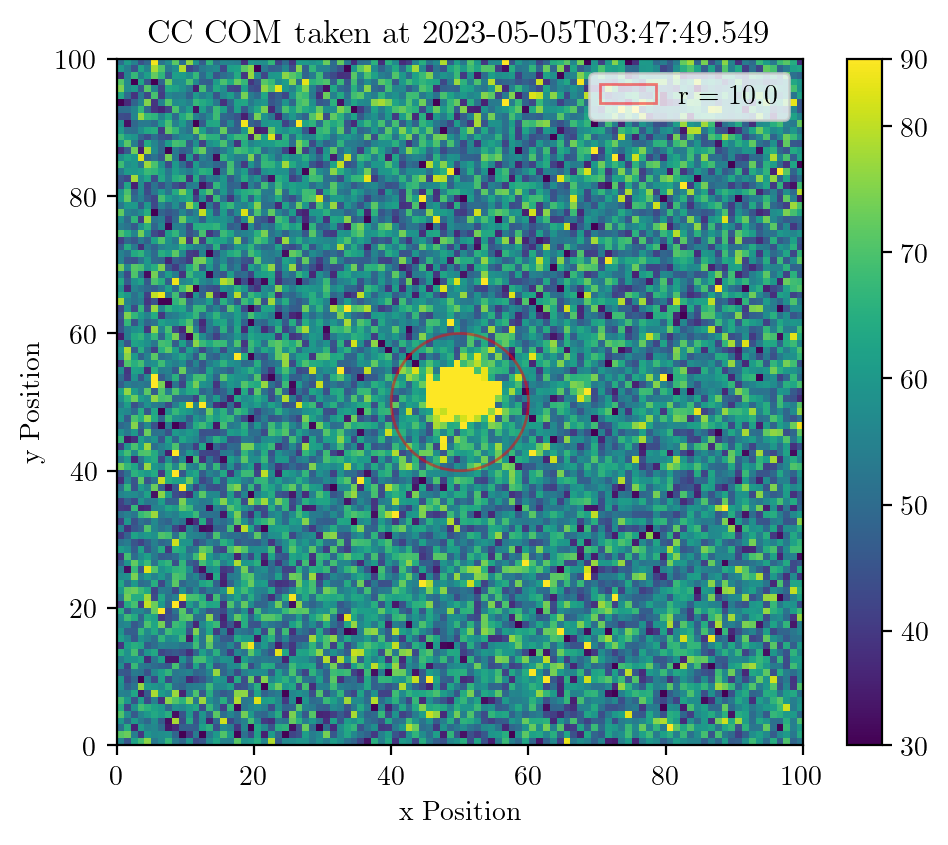
\includegraphics[width=0.7\textwidth]{figures/cc-com_reduced-example.png}
        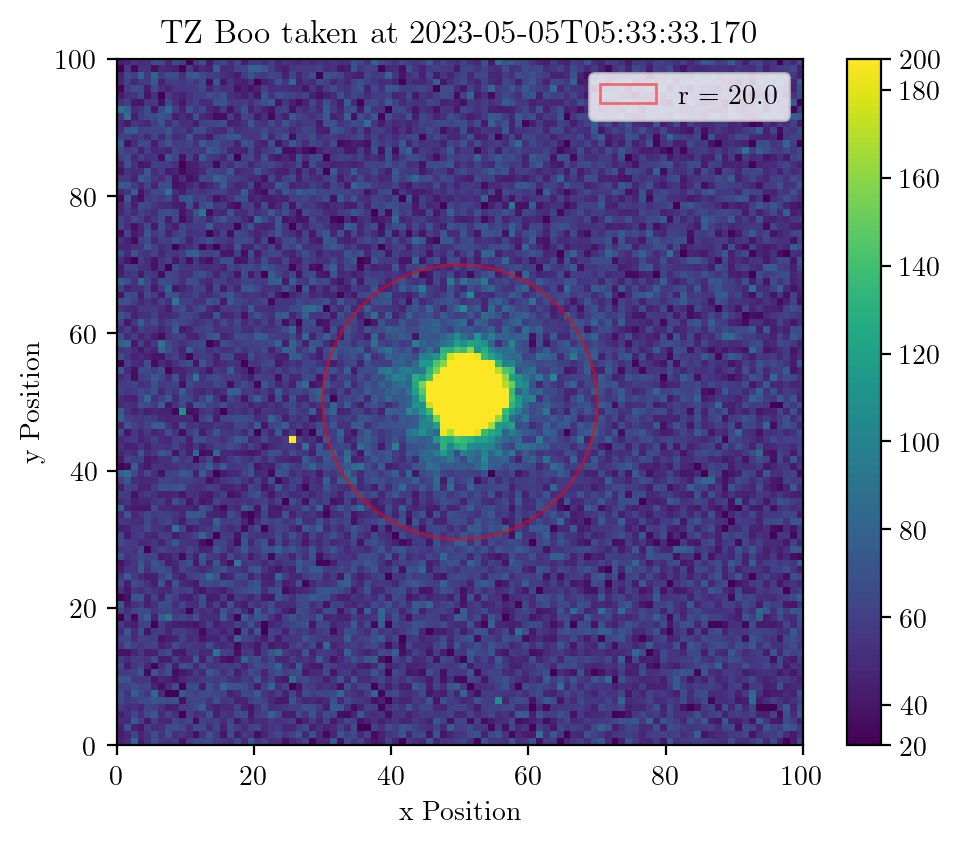
\includegraphics[width=0.7\textwidth]{figures/tz-boo_reduced-example.png}
    \end{center}
    \caption{Images of V* CC Com and TZ Boo post-reduction. A circular aperture can consistently capture the shape of both star systems.}
\end{figure}

\section{Data Analysis}

\subsection{Discussion of Fitting Methods}

Markov Chain Monte Carlo (MCMC) algorithms are particularly well-suited for analyzing time series data because they can handle complex models and incorporate uncertainties in the observed data and model parameters. In the context of eclipsing binary stars, MCMC can be used to estimate the parameters that describe the physical properties of the stars and their orbit.

MCMC is useful for our project as it is an effective tool for determining the fit parameters for light curve data, including calculation of the orbital period. Generally, the curves for time series analyses involve many parameters requiring adjustment to the observed data. This would be otherwise computationally expensive due to the high amount of dimensions needed to compute.

However, due to the low count of data points we were able to obtain for either star system, we decided against using MCMC methods. MCMC methods require much higher data point count in order to reduce the uncertainty in the fit results. Additionally, it is difficult to determine whether MCMC methods have ``converged’’ onto a result, especially with a limited supply of data points.

Another method we considered to work with our relatively low data point count was using the \codeword{lmfit} python package. \codeword{lmfit} presents various regression analysis tools, including a sinusoidal model. Despite the package’s capabilities in accommodating a lower data point count than MCMC methods, the sinusoidal model had difficulties fitting with the given datasets. We attribute this difficulty to the ambiguity of where the data points exist on a given sinusoid. A string of data points could exist on the trough or a crest of a curve. Had we observed a longer portion of a period for our star systems, this ambiguity could have been reduced.


We eventually estimated the period of the dataset by approximating a crest/trough of a sinusoid via Taylor expansion. Given a fit model curve of
\begin{equation}
    f(t) = \frac{1}{2}\left(1 + \cos\left(\frac{2\pi}{P} (t - \phi) \right)\right)
\end{equation} 
where $P$ is the orbital period of the eclipsing binary system, we can estimate the fit model curve via a second order Taylor expansion, 

\begin{equation}
    f(t) \approx 1 - \frac{1}{4}\left( \frac{2\pi}{P}(t - \phi) \right)^{2} = 1 - \frac{\pi^2}{P^2}\left( t - \phi \right) ^2
\end{equation} 

The data points were fit to a quadratic model curve of the form $at^2 + bt + c$. This means that the period $P$ has the following relation $P=\sqrt{\pi^2 / a} $. By experimentation, this approximation was more effective in estimating the light curve than the built-in sinusoidal model in \codeword{lmfit}.

\section{Discussion of Results}

\subsection{Observation Data}

\begin{table}[htpb]
\centering
\begin{tabular}{lllll}
    \toprule
\textbf{Time} & \textbf{Centroid} $(x, y)$ & \textbf{DAO Flux} & \textbf{AP Flux} \\
\midrule
03:37:43.990  & (1505.659, 1451.960)                     & 45.284            & 162209                            \\
04:06:02.330  & (1486.507, 1459.452)                     & 70.992            & 176519                            \\
04:33:47.270  & (1529.808, 1527.439)                     & 128.777           & 182434                            \\
05:33:33.170  & (1524.298, 1521.622)                     & 102.930           & 159071                           \\
\bottomrule
\end{tabular}
\caption{V* TZ Boo observation data taken on May 05, 2023. Exposure time for all images was \SI{15}{\s} and aperture radius 20.0 px.}
\end{table}

\begin{table}[htpb]
\centering
\begin{tabular}{lllllll}
    \toprule
\textbf{Time} & \textbf{Centroid} $(x, y)$ & \textbf{DAO Flux} & \textbf{AP Flux} \\
\midrule
03:47:49.549  & (1553.040, 1437.503)                     & 3.312             & 8869      \\
04:15:01.570  & (1551.455, 1438.762)                     & 4.400             & 9698                              \\
04:58:12.580  & (1550.136, 1438.673)                     & 5.942             & 9392                              \\
\bottomrule
\end{tabular}
\caption{V* CC Com observation data taken on May 05, 2023. Exposure time for all images was \SI{15}{\s} and aperture radius 20.0 px.}
\end{table}
\subsection{Curve Fit Data}
\begin{figure}[htpb]
    \begin{center}
        %% Creator: Matplotlib, PGF backend
%%
%% To include the figure in your LaTeX document, write
%%   \input{<filename>.pgf}
%%
%% Make sure the required packages are loaded in your preamble
%%   \usepackage{pgf}
%%
%% Also ensure that all the required font packages are loaded; for instance,
%% the lmodern package is sometimes necessary when using math font.
%%   \usepackage{lmodern}
%%
%% Figures using additional raster images can only be included by \input if
%% they are in the same directory as the main LaTeX file. For loading figures
%% from other directories you can use the `import` package
%%   \usepackage{import}
%%
%% and then include the figures with
%%   \import{<path to file>}{<filename>.pgf}
%%
%% Matplotlib used the following preamble
%%
\begingroup%
\makeatletter%
\begin{pgfpicture}%
\pgfpathrectangle{\pgfpointorigin}{\pgfqpoint{5.000000in}{3.800000in}}%
\pgfusepath{use as bounding box, clip}%
\begin{pgfscope}%
\pgfsetbuttcap%
\pgfsetmiterjoin%
\pgfsetlinewidth{0.000000pt}%
\definecolor{currentstroke}{rgb}{1.000000,1.000000,1.000000}%
\pgfsetstrokecolor{currentstroke}%
\pgfsetstrokeopacity{0.000000}%
\pgfsetdash{}{0pt}%
\pgfpathmoveto{\pgfqpoint{0.000000in}{0.000000in}}%
\pgfpathlineto{\pgfqpoint{5.000000in}{0.000000in}}%
\pgfpathlineto{\pgfqpoint{5.000000in}{3.800000in}}%
\pgfpathlineto{\pgfqpoint{0.000000in}{3.800000in}}%
\pgfpathlineto{\pgfqpoint{0.000000in}{0.000000in}}%
\pgfpathclose%
\pgfusepath{}%
\end{pgfscope}%
\begin{pgfscope}%
\pgfsetbuttcap%
\pgfsetmiterjoin%
\definecolor{currentfill}{rgb}{1.000000,1.000000,1.000000}%
\pgfsetfillcolor{currentfill}%
\pgfsetlinewidth{0.000000pt}%
\definecolor{currentstroke}{rgb}{0.000000,0.000000,0.000000}%
\pgfsetstrokecolor{currentstroke}%
\pgfsetstrokeopacity{0.000000}%
\pgfsetdash{}{0pt}%
\pgfpathmoveto{\pgfqpoint{0.625000in}{0.475000in}}%
\pgfpathlineto{\pgfqpoint{4.500000in}{0.475000in}}%
\pgfpathlineto{\pgfqpoint{4.500000in}{3.344000in}}%
\pgfpathlineto{\pgfqpoint{0.625000in}{3.344000in}}%
\pgfpathlineto{\pgfqpoint{0.625000in}{0.475000in}}%
\pgfpathclose%
\pgfusepath{fill}%
\end{pgfscope}%
\begin{pgfscope}%
\pgfpathrectangle{\pgfqpoint{0.625000in}{0.475000in}}{\pgfqpoint{3.875000in}{2.869000in}}%
\pgfusepath{clip}%
\pgfsetbuttcap%
\pgfsetroundjoin%
\definecolor{currentfill}{rgb}{0.121569,0.466667,0.705882}%
\pgfsetfillcolor{currentfill}%
\pgfsetlinewidth{1.003750pt}%
\definecolor{currentstroke}{rgb}{0.121569,0.466667,0.705882}%
\pgfsetstrokecolor{currentstroke}%
\pgfsetdash{}{0pt}%
\pgfsys@defobject{currentmarker}{\pgfqpoint{-0.041667in}{-0.041667in}}{\pgfqpoint{0.041667in}{0.041667in}}{%
\pgfpathmoveto{\pgfqpoint{0.000000in}{-0.041667in}}%
\pgfpathcurveto{\pgfqpoint{0.011050in}{-0.041667in}}{\pgfqpoint{0.021649in}{-0.037276in}}{\pgfqpoint{0.029463in}{-0.029463in}}%
\pgfpathcurveto{\pgfqpoint{0.037276in}{-0.021649in}}{\pgfqpoint{0.041667in}{-0.011050in}}{\pgfqpoint{0.041667in}{0.000000in}}%
\pgfpathcurveto{\pgfqpoint{0.041667in}{0.011050in}}{\pgfqpoint{0.037276in}{0.021649in}}{\pgfqpoint{0.029463in}{0.029463in}}%
\pgfpathcurveto{\pgfqpoint{0.021649in}{0.037276in}}{\pgfqpoint{0.011050in}{0.041667in}}{\pgfqpoint{0.000000in}{0.041667in}}%
\pgfpathcurveto{\pgfqpoint{-0.011050in}{0.041667in}}{\pgfqpoint{-0.021649in}{0.037276in}}{\pgfqpoint{-0.029463in}{0.029463in}}%
\pgfpathcurveto{\pgfqpoint{-0.037276in}{0.021649in}}{\pgfqpoint{-0.041667in}{0.011050in}}{\pgfqpoint{-0.041667in}{0.000000in}}%
\pgfpathcurveto{\pgfqpoint{-0.041667in}{-0.011050in}}{\pgfqpoint{-0.037276in}{-0.021649in}}{\pgfqpoint{-0.029463in}{-0.029463in}}%
\pgfpathcurveto{\pgfqpoint{-0.021649in}{-0.037276in}}{\pgfqpoint{-0.011050in}{-0.041667in}}{\pgfqpoint{0.000000in}{-0.041667in}}%
\pgfpathlineto{\pgfqpoint{0.000000in}{-0.041667in}}%
\pgfpathclose%
\pgfusepath{stroke,fill}%
}%
\begin{pgfscope}%
\pgfsys@transformshift{2.562500in}{2.294171in}%
\pgfsys@useobject{currentmarker}{}%
\end{pgfscope}%
\begin{pgfscope}%
\pgfsys@transformshift{2.713046in}{2.447437in}%
\pgfsys@useobject{currentmarker}{}%
\end{pgfscope}%
\begin{pgfscope}%
\pgfsys@transformshift{2.952054in}{2.390994in}%
\pgfsys@useobject{currentmarker}{}%
\end{pgfscope}%
\end{pgfscope}%
\begin{pgfscope}%
\pgfsetbuttcap%
\pgfsetroundjoin%
\definecolor{currentfill}{rgb}{0.000000,0.000000,0.000000}%
\pgfsetfillcolor{currentfill}%
\pgfsetlinewidth{0.803000pt}%
\definecolor{currentstroke}{rgb}{0.000000,0.000000,0.000000}%
\pgfsetstrokecolor{currentstroke}%
\pgfsetdash{}{0pt}%
\pgfsys@defobject{currentmarker}{\pgfqpoint{0.000000in}{-0.048611in}}{\pgfqpoint{0.000000in}{0.000000in}}{%
\pgfpathmoveto{\pgfqpoint{0.000000in}{0.000000in}}%
\pgfpathlineto{\pgfqpoint{0.000000in}{-0.048611in}}%
\pgfusepath{stroke,fill}%
}%
\begin{pgfscope}%
\pgfsys@transformshift{0.968506in}{0.475000in}%
\pgfsys@useobject{currentmarker}{}%
\end{pgfscope}%
\end{pgfscope}%
\begin{pgfscope}%
\definecolor{textcolor}{rgb}{0.000000,0.000000,0.000000}%
\pgfsetstrokecolor{textcolor}%
\pgfsetfillcolor{textcolor}%
\pgftext[x=0.968506in,y=0.377778in,,top]{\color{textcolor}\rmfamily\fontsize{10.000000}{12.000000}\selectfont \(\displaystyle {\ensuremath{-}0.2}\)}%
\end{pgfscope}%
\begin{pgfscope}%
\pgfsetbuttcap%
\pgfsetroundjoin%
\definecolor{currentfill}{rgb}{0.000000,0.000000,0.000000}%
\pgfsetfillcolor{currentfill}%
\pgfsetlinewidth{0.803000pt}%
\definecolor{currentstroke}{rgb}{0.000000,0.000000,0.000000}%
\pgfsetstrokecolor{currentstroke}%
\pgfsetdash{}{0pt}%
\pgfsys@defobject{currentmarker}{\pgfqpoint{0.000000in}{-0.048611in}}{\pgfqpoint{0.000000in}{0.000000in}}{%
\pgfpathmoveto{\pgfqpoint{0.000000in}{0.000000in}}%
\pgfpathlineto{\pgfqpoint{0.000000in}{-0.048611in}}%
\pgfusepath{stroke,fill}%
}%
\begin{pgfscope}%
\pgfsys@transformshift{1.765503in}{0.475000in}%
\pgfsys@useobject{currentmarker}{}%
\end{pgfscope}%
\end{pgfscope}%
\begin{pgfscope}%
\definecolor{textcolor}{rgb}{0.000000,0.000000,0.000000}%
\pgfsetstrokecolor{textcolor}%
\pgfsetfillcolor{textcolor}%
\pgftext[x=1.765503in,y=0.377778in,,top]{\color{textcolor}\rmfamily\fontsize{10.000000}{12.000000}\selectfont \(\displaystyle {\ensuremath{-}0.1}\)}%
\end{pgfscope}%
\begin{pgfscope}%
\pgfsetbuttcap%
\pgfsetroundjoin%
\definecolor{currentfill}{rgb}{0.000000,0.000000,0.000000}%
\pgfsetfillcolor{currentfill}%
\pgfsetlinewidth{0.803000pt}%
\definecolor{currentstroke}{rgb}{0.000000,0.000000,0.000000}%
\pgfsetstrokecolor{currentstroke}%
\pgfsetdash{}{0pt}%
\pgfsys@defobject{currentmarker}{\pgfqpoint{0.000000in}{-0.048611in}}{\pgfqpoint{0.000000in}{0.000000in}}{%
\pgfpathmoveto{\pgfqpoint{0.000000in}{0.000000in}}%
\pgfpathlineto{\pgfqpoint{0.000000in}{-0.048611in}}%
\pgfusepath{stroke,fill}%
}%
\begin{pgfscope}%
\pgfsys@transformshift{2.562500in}{0.475000in}%
\pgfsys@useobject{currentmarker}{}%
\end{pgfscope}%
\end{pgfscope}%
\begin{pgfscope}%
\definecolor{textcolor}{rgb}{0.000000,0.000000,0.000000}%
\pgfsetstrokecolor{textcolor}%
\pgfsetfillcolor{textcolor}%
\pgftext[x=2.562500in,y=0.377778in,,top]{\color{textcolor}\rmfamily\fontsize{10.000000}{12.000000}\selectfont \(\displaystyle {0.0}\)}%
\end{pgfscope}%
\begin{pgfscope}%
\pgfsetbuttcap%
\pgfsetroundjoin%
\definecolor{currentfill}{rgb}{0.000000,0.000000,0.000000}%
\pgfsetfillcolor{currentfill}%
\pgfsetlinewidth{0.803000pt}%
\definecolor{currentstroke}{rgb}{0.000000,0.000000,0.000000}%
\pgfsetstrokecolor{currentstroke}%
\pgfsetdash{}{0pt}%
\pgfsys@defobject{currentmarker}{\pgfqpoint{0.000000in}{-0.048611in}}{\pgfqpoint{0.000000in}{0.000000in}}{%
\pgfpathmoveto{\pgfqpoint{0.000000in}{0.000000in}}%
\pgfpathlineto{\pgfqpoint{0.000000in}{-0.048611in}}%
\pgfusepath{stroke,fill}%
}%
\begin{pgfscope}%
\pgfsys@transformshift{3.359497in}{0.475000in}%
\pgfsys@useobject{currentmarker}{}%
\end{pgfscope}%
\end{pgfscope}%
\begin{pgfscope}%
\definecolor{textcolor}{rgb}{0.000000,0.000000,0.000000}%
\pgfsetstrokecolor{textcolor}%
\pgfsetfillcolor{textcolor}%
\pgftext[x=3.359497in,y=0.377778in,,top]{\color{textcolor}\rmfamily\fontsize{10.000000}{12.000000}\selectfont \(\displaystyle {0.1}\)}%
\end{pgfscope}%
\begin{pgfscope}%
\pgfsetbuttcap%
\pgfsetroundjoin%
\definecolor{currentfill}{rgb}{0.000000,0.000000,0.000000}%
\pgfsetfillcolor{currentfill}%
\pgfsetlinewidth{0.803000pt}%
\definecolor{currentstroke}{rgb}{0.000000,0.000000,0.000000}%
\pgfsetstrokecolor{currentstroke}%
\pgfsetdash{}{0pt}%
\pgfsys@defobject{currentmarker}{\pgfqpoint{0.000000in}{-0.048611in}}{\pgfqpoint{0.000000in}{0.000000in}}{%
\pgfpathmoveto{\pgfqpoint{0.000000in}{0.000000in}}%
\pgfpathlineto{\pgfqpoint{0.000000in}{-0.048611in}}%
\pgfusepath{stroke,fill}%
}%
\begin{pgfscope}%
\pgfsys@transformshift{4.156494in}{0.475000in}%
\pgfsys@useobject{currentmarker}{}%
\end{pgfscope}%
\end{pgfscope}%
\begin{pgfscope}%
\definecolor{textcolor}{rgb}{0.000000,0.000000,0.000000}%
\pgfsetstrokecolor{textcolor}%
\pgfsetfillcolor{textcolor}%
\pgftext[x=4.156494in,y=0.377778in,,top]{\color{textcolor}\rmfamily\fontsize{10.000000}{12.000000}\selectfont \(\displaystyle {0.2}\)}%
\end{pgfscope}%
\begin{pgfscope}%
\definecolor{textcolor}{rgb}{0.000000,0.000000,0.000000}%
\pgfsetstrokecolor{textcolor}%
\pgfsetfillcolor{textcolor}%
\pgftext[x=2.562500in,y=0.198766in,,top]{\color{textcolor}\rmfamily\fontsize{10.000000}{12.000000}\selectfont Phase [d]}%
\end{pgfscope}%
\begin{pgfscope}%
\pgfsetbuttcap%
\pgfsetroundjoin%
\definecolor{currentfill}{rgb}{0.000000,0.000000,0.000000}%
\pgfsetfillcolor{currentfill}%
\pgfsetlinewidth{0.803000pt}%
\definecolor{currentstroke}{rgb}{0.000000,0.000000,0.000000}%
\pgfsetstrokecolor{currentstroke}%
\pgfsetdash{}{0pt}%
\pgfsys@defobject{currentmarker}{\pgfqpoint{-0.048611in}{0.000000in}}{\pgfqpoint{-0.000000in}{0.000000in}}{%
\pgfpathmoveto{\pgfqpoint{-0.000000in}{0.000000in}}%
\pgfpathlineto{\pgfqpoint{-0.048611in}{0.000000in}}%
\pgfusepath{stroke,fill}%
}%
\begin{pgfscope}%
\pgfsys@transformshift{0.625000in}{0.654313in}%
\pgfsys@useobject{currentmarker}{}%
\end{pgfscope}%
\end{pgfscope}%
\begin{pgfscope}%
\definecolor{textcolor}{rgb}{0.000000,0.000000,0.000000}%
\pgfsetstrokecolor{textcolor}%
\pgfsetfillcolor{textcolor}%
\pgftext[x=0.350308in, y=0.606087in, left, base]{\color{textcolor}\rmfamily\fontsize{10.000000}{12.000000}\selectfont \(\displaystyle {0.0}\)}%
\end{pgfscope}%
\begin{pgfscope}%
\pgfsetbuttcap%
\pgfsetroundjoin%
\definecolor{currentfill}{rgb}{0.000000,0.000000,0.000000}%
\pgfsetfillcolor{currentfill}%
\pgfsetlinewidth{0.803000pt}%
\definecolor{currentstroke}{rgb}{0.000000,0.000000,0.000000}%
\pgfsetstrokecolor{currentstroke}%
\pgfsetdash{}{0pt}%
\pgfsys@defobject{currentmarker}{\pgfqpoint{-0.048611in}{0.000000in}}{\pgfqpoint{-0.000000in}{0.000000in}}{%
\pgfpathmoveto{\pgfqpoint{-0.000000in}{0.000000in}}%
\pgfpathlineto{\pgfqpoint{-0.048611in}{0.000000in}}%
\pgfusepath{stroke,fill}%
}%
\begin{pgfscope}%
\pgfsys@transformshift{0.625000in}{1.012938in}%
\pgfsys@useobject{currentmarker}{}%
\end{pgfscope}%
\end{pgfscope}%
\begin{pgfscope}%
\definecolor{textcolor}{rgb}{0.000000,0.000000,0.000000}%
\pgfsetstrokecolor{textcolor}%
\pgfsetfillcolor{textcolor}%
\pgftext[x=0.350308in, y=0.964712in, left, base]{\color{textcolor}\rmfamily\fontsize{10.000000}{12.000000}\selectfont \(\displaystyle {0.2}\)}%
\end{pgfscope}%
\begin{pgfscope}%
\pgfsetbuttcap%
\pgfsetroundjoin%
\definecolor{currentfill}{rgb}{0.000000,0.000000,0.000000}%
\pgfsetfillcolor{currentfill}%
\pgfsetlinewidth{0.803000pt}%
\definecolor{currentstroke}{rgb}{0.000000,0.000000,0.000000}%
\pgfsetstrokecolor{currentstroke}%
\pgfsetdash{}{0pt}%
\pgfsys@defobject{currentmarker}{\pgfqpoint{-0.048611in}{0.000000in}}{\pgfqpoint{-0.000000in}{0.000000in}}{%
\pgfpathmoveto{\pgfqpoint{-0.000000in}{0.000000in}}%
\pgfpathlineto{\pgfqpoint{-0.048611in}{0.000000in}}%
\pgfusepath{stroke,fill}%
}%
\begin{pgfscope}%
\pgfsys@transformshift{0.625000in}{1.371563in}%
\pgfsys@useobject{currentmarker}{}%
\end{pgfscope}%
\end{pgfscope}%
\begin{pgfscope}%
\definecolor{textcolor}{rgb}{0.000000,0.000000,0.000000}%
\pgfsetstrokecolor{textcolor}%
\pgfsetfillcolor{textcolor}%
\pgftext[x=0.350308in, y=1.323337in, left, base]{\color{textcolor}\rmfamily\fontsize{10.000000}{12.000000}\selectfont \(\displaystyle {0.4}\)}%
\end{pgfscope}%
\begin{pgfscope}%
\pgfsetbuttcap%
\pgfsetroundjoin%
\definecolor{currentfill}{rgb}{0.000000,0.000000,0.000000}%
\pgfsetfillcolor{currentfill}%
\pgfsetlinewidth{0.803000pt}%
\definecolor{currentstroke}{rgb}{0.000000,0.000000,0.000000}%
\pgfsetstrokecolor{currentstroke}%
\pgfsetdash{}{0pt}%
\pgfsys@defobject{currentmarker}{\pgfqpoint{-0.048611in}{0.000000in}}{\pgfqpoint{-0.000000in}{0.000000in}}{%
\pgfpathmoveto{\pgfqpoint{-0.000000in}{0.000000in}}%
\pgfpathlineto{\pgfqpoint{-0.048611in}{0.000000in}}%
\pgfusepath{stroke,fill}%
}%
\begin{pgfscope}%
\pgfsys@transformshift{0.625000in}{1.730188in}%
\pgfsys@useobject{currentmarker}{}%
\end{pgfscope}%
\end{pgfscope}%
\begin{pgfscope}%
\definecolor{textcolor}{rgb}{0.000000,0.000000,0.000000}%
\pgfsetstrokecolor{textcolor}%
\pgfsetfillcolor{textcolor}%
\pgftext[x=0.350308in, y=1.681962in, left, base]{\color{textcolor}\rmfamily\fontsize{10.000000}{12.000000}\selectfont \(\displaystyle {0.6}\)}%
\end{pgfscope}%
\begin{pgfscope}%
\pgfsetbuttcap%
\pgfsetroundjoin%
\definecolor{currentfill}{rgb}{0.000000,0.000000,0.000000}%
\pgfsetfillcolor{currentfill}%
\pgfsetlinewidth{0.803000pt}%
\definecolor{currentstroke}{rgb}{0.000000,0.000000,0.000000}%
\pgfsetstrokecolor{currentstroke}%
\pgfsetdash{}{0pt}%
\pgfsys@defobject{currentmarker}{\pgfqpoint{-0.048611in}{0.000000in}}{\pgfqpoint{-0.000000in}{0.000000in}}{%
\pgfpathmoveto{\pgfqpoint{-0.000000in}{0.000000in}}%
\pgfpathlineto{\pgfqpoint{-0.048611in}{0.000000in}}%
\pgfusepath{stroke,fill}%
}%
\begin{pgfscope}%
\pgfsys@transformshift{0.625000in}{2.088813in}%
\pgfsys@useobject{currentmarker}{}%
\end{pgfscope}%
\end{pgfscope}%
\begin{pgfscope}%
\definecolor{textcolor}{rgb}{0.000000,0.000000,0.000000}%
\pgfsetstrokecolor{textcolor}%
\pgfsetfillcolor{textcolor}%
\pgftext[x=0.350308in, y=2.040587in, left, base]{\color{textcolor}\rmfamily\fontsize{10.000000}{12.000000}\selectfont \(\displaystyle {0.8}\)}%
\end{pgfscope}%
\begin{pgfscope}%
\pgfsetbuttcap%
\pgfsetroundjoin%
\definecolor{currentfill}{rgb}{0.000000,0.000000,0.000000}%
\pgfsetfillcolor{currentfill}%
\pgfsetlinewidth{0.803000pt}%
\definecolor{currentstroke}{rgb}{0.000000,0.000000,0.000000}%
\pgfsetstrokecolor{currentstroke}%
\pgfsetdash{}{0pt}%
\pgfsys@defobject{currentmarker}{\pgfqpoint{-0.048611in}{0.000000in}}{\pgfqpoint{-0.000000in}{0.000000in}}{%
\pgfpathmoveto{\pgfqpoint{-0.000000in}{0.000000in}}%
\pgfpathlineto{\pgfqpoint{-0.048611in}{0.000000in}}%
\pgfusepath{stroke,fill}%
}%
\begin{pgfscope}%
\pgfsys@transformshift{0.625000in}{2.447438in}%
\pgfsys@useobject{currentmarker}{}%
\end{pgfscope}%
\end{pgfscope}%
\begin{pgfscope}%
\definecolor{textcolor}{rgb}{0.000000,0.000000,0.000000}%
\pgfsetstrokecolor{textcolor}%
\pgfsetfillcolor{textcolor}%
\pgftext[x=0.350308in, y=2.399212in, left, base]{\color{textcolor}\rmfamily\fontsize{10.000000}{12.000000}\selectfont \(\displaystyle {1.0}\)}%
\end{pgfscope}%
\begin{pgfscope}%
\pgfsetbuttcap%
\pgfsetroundjoin%
\definecolor{currentfill}{rgb}{0.000000,0.000000,0.000000}%
\pgfsetfillcolor{currentfill}%
\pgfsetlinewidth{0.803000pt}%
\definecolor{currentstroke}{rgb}{0.000000,0.000000,0.000000}%
\pgfsetstrokecolor{currentstroke}%
\pgfsetdash{}{0pt}%
\pgfsys@defobject{currentmarker}{\pgfqpoint{-0.048611in}{0.000000in}}{\pgfqpoint{-0.000000in}{0.000000in}}{%
\pgfpathmoveto{\pgfqpoint{-0.000000in}{0.000000in}}%
\pgfpathlineto{\pgfqpoint{-0.048611in}{0.000000in}}%
\pgfusepath{stroke,fill}%
}%
\begin{pgfscope}%
\pgfsys@transformshift{0.625000in}{2.806063in}%
\pgfsys@useobject{currentmarker}{}%
\end{pgfscope}%
\end{pgfscope}%
\begin{pgfscope}%
\definecolor{textcolor}{rgb}{0.000000,0.000000,0.000000}%
\pgfsetstrokecolor{textcolor}%
\pgfsetfillcolor{textcolor}%
\pgftext[x=0.350308in, y=2.757837in, left, base]{\color{textcolor}\rmfamily\fontsize{10.000000}{12.000000}\selectfont \(\displaystyle {1.2}\)}%
\end{pgfscope}%
\begin{pgfscope}%
\pgfsetbuttcap%
\pgfsetroundjoin%
\definecolor{currentfill}{rgb}{0.000000,0.000000,0.000000}%
\pgfsetfillcolor{currentfill}%
\pgfsetlinewidth{0.803000pt}%
\definecolor{currentstroke}{rgb}{0.000000,0.000000,0.000000}%
\pgfsetstrokecolor{currentstroke}%
\pgfsetdash{}{0pt}%
\pgfsys@defobject{currentmarker}{\pgfqpoint{-0.048611in}{0.000000in}}{\pgfqpoint{-0.000000in}{0.000000in}}{%
\pgfpathmoveto{\pgfqpoint{-0.000000in}{0.000000in}}%
\pgfpathlineto{\pgfqpoint{-0.048611in}{0.000000in}}%
\pgfusepath{stroke,fill}%
}%
\begin{pgfscope}%
\pgfsys@transformshift{0.625000in}{3.164687in}%
\pgfsys@useobject{currentmarker}{}%
\end{pgfscope}%
\end{pgfscope}%
\begin{pgfscope}%
\definecolor{textcolor}{rgb}{0.000000,0.000000,0.000000}%
\pgfsetstrokecolor{textcolor}%
\pgfsetfillcolor{textcolor}%
\pgftext[x=0.350308in, y=3.116462in, left, base]{\color{textcolor}\rmfamily\fontsize{10.000000}{12.000000}\selectfont \(\displaystyle {1.4}\)}%
\end{pgfscope}%
\begin{pgfscope}%
\definecolor{textcolor}{rgb}{0.000000,0.000000,0.000000}%
\pgfsetstrokecolor{textcolor}%
\pgfsetfillcolor{textcolor}%
\pgftext[x=0.294753in,y=1.909500in,,bottom,rotate=90.000000]{\color{textcolor}\rmfamily\fontsize{10.000000}{12.000000}\selectfont Normalized Flux}%
\end{pgfscope}%
\begin{pgfscope}%
\pgfpathrectangle{\pgfqpoint{0.625000in}{0.475000in}}{\pgfqpoint{3.875000in}{2.869000in}}%
\pgfusepath{clip}%
\pgfsetrectcap%
\pgfsetroundjoin%
\pgfsetlinewidth{1.505625pt}%
\definecolor{currentstroke}{rgb}{0.121569,0.466667,0.705882}%
\pgfsetstrokecolor{currentstroke}%
\pgfsetdash{}{0pt}%
\pgfpathmoveto{\pgfqpoint{0.801136in}{2.140621in}}%
\pgfpathlineto{\pgfqpoint{0.836719in}{2.221364in}}%
\pgfpathlineto{\pgfqpoint{0.872303in}{2.291318in}}%
\pgfpathlineto{\pgfqpoint{0.907886in}{2.349358in}}%
\pgfpathlineto{\pgfqpoint{0.943469in}{2.394551in}}%
\pgfpathlineto{\pgfqpoint{0.979052in}{2.426168in}}%
\pgfpathlineto{\pgfqpoint{1.014635in}{2.443701in}}%
\pgfpathlineto{\pgfqpoint{1.050218in}{2.446869in}}%
\pgfpathlineto{\pgfqpoint{1.085801in}{2.435620in}}%
\pgfpathlineto{\pgfqpoint{1.121384in}{2.410135in}}%
\pgfpathlineto{\pgfqpoint{1.156967in}{2.370824in}}%
\pgfpathlineto{\pgfqpoint{1.192551in}{2.318319in}}%
\pgfpathlineto{\pgfqpoint{1.228134in}{2.253467in}}%
\pgfpathlineto{\pgfqpoint{1.263717in}{2.177309in}}%
\pgfpathlineto{\pgfqpoint{1.299300in}{2.091072in}}%
\pgfpathlineto{\pgfqpoint{1.334883in}{1.996143in}}%
\pgfpathlineto{\pgfqpoint{1.370466in}{1.894049in}}%
\pgfpathlineto{\pgfqpoint{1.406049in}{1.786433in}}%
\pgfpathlineto{\pgfqpoint{1.441632in}{1.675028in}}%
\pgfpathlineto{\pgfqpoint{1.477215in}{1.561624in}}%
\pgfpathlineto{\pgfqpoint{1.512798in}{1.448048in}}%
\pgfpathlineto{\pgfqpoint{1.548382in}{1.336126in}}%
\pgfpathlineto{\pgfqpoint{1.583965in}{1.227660in}}%
\pgfpathlineto{\pgfqpoint{1.619548in}{1.124394in}}%
\pgfpathlineto{\pgfqpoint{1.655131in}{1.027990in}}%
\pgfpathlineto{\pgfqpoint{1.690714in}{0.940000in}}%
\pgfpathlineto{\pgfqpoint{1.726297in}{0.861839in}}%
\pgfpathlineto{\pgfqpoint{1.761880in}{0.794765in}}%
\pgfpathlineto{\pgfqpoint{1.797463in}{0.739857in}}%
\pgfpathlineto{\pgfqpoint{1.833046in}{0.697999in}}%
\pgfpathlineto{\pgfqpoint{1.868629in}{0.669863in}}%
\pgfpathlineto{\pgfqpoint{1.904213in}{0.655904in}}%
\pgfpathlineto{\pgfqpoint{1.939796in}{0.656345in}}%
\pgfpathlineto{\pgfqpoint{1.975379in}{0.671179in}}%
\pgfpathlineto{\pgfqpoint{2.010962in}{0.700168in}}%
\pgfpathlineto{\pgfqpoint{2.046545in}{0.742845in}}%
\pgfpathlineto{\pgfqpoint{2.082128in}{0.798524in}}%
\pgfpathlineto{\pgfqpoint{2.117711in}{0.866308in}}%
\pgfpathlineto{\pgfqpoint{2.153294in}{0.945107in}}%
\pgfpathlineto{\pgfqpoint{2.188877in}{1.033653in}}%
\pgfpathlineto{\pgfqpoint{2.224461in}{1.130521in}}%
\pgfpathlineto{\pgfqpoint{2.260044in}{1.234154in}}%
\pgfpathlineto{\pgfqpoint{2.295627in}{1.342882in}}%
\pgfpathlineto{\pgfqpoint{2.331210in}{1.454957in}}%
\pgfpathlineto{\pgfqpoint{2.366793in}{1.568575in}}%
\pgfpathlineto{\pgfqpoint{2.402376in}{1.681909in}}%
\pgfpathlineto{\pgfqpoint{2.437959in}{1.793134in}}%
\pgfpathlineto{\pgfqpoint{2.473542in}{1.900461in}}%
\pgfpathlineto{\pgfqpoint{2.509125in}{2.002163in}}%
\pgfpathlineto{\pgfqpoint{2.544708in}{2.096604in}}%
\pgfpathlineto{\pgfqpoint{2.580292in}{2.182264in}}%
\pgfpathlineto{\pgfqpoint{2.615875in}{2.257764in}}%
\pgfpathlineto{\pgfqpoint{2.651458in}{2.321890in}}%
\pgfpathlineto{\pgfqpoint{2.687041in}{2.373611in}}%
\pgfpathlineto{\pgfqpoint{2.722624in}{2.412093in}}%
\pgfpathlineto{\pgfqpoint{2.758207in}{2.436718in}}%
\pgfpathlineto{\pgfqpoint{2.793790in}{2.447090in}}%
\pgfpathlineto{\pgfqpoint{2.829373in}{2.443041in}}%
\pgfpathlineto{\pgfqpoint{2.864956in}{2.424636in}}%
\pgfpathlineto{\pgfqpoint{2.900539in}{2.392173in}}%
\pgfpathlineto{\pgfqpoint{2.936123in}{2.346173in}}%
\pgfpathlineto{\pgfqpoint{2.971706in}{2.287376in}}%
\pgfpathlineto{\pgfqpoint{3.007289in}{2.216729in}}%
\pgfpathlineto{\pgfqpoint{3.042872in}{2.135367in}}%
\pgfpathlineto{\pgfqpoint{3.078455in}{2.044601in}}%
\pgfpathlineto{\pgfqpoint{3.114038in}{1.945891in}}%
\pgfpathlineto{\pgfqpoint{3.149621in}{1.840825in}}%
\pgfpathlineto{\pgfqpoint{3.185204in}{1.731093in}}%
\pgfpathlineto{\pgfqpoint{3.220787in}{1.618462in}}%
\pgfpathlineto{\pgfqpoint{3.256371in}{1.504743in}}%
\pgfpathlineto{\pgfqpoint{3.291954in}{1.391767in}}%
\pgfpathlineto{\pgfqpoint{3.327537in}{1.281350in}}%
\pgfpathlineto{\pgfqpoint{3.363120in}{1.175270in}}%
\pgfpathlineto{\pgfqpoint{3.398703in}{1.075234in}}%
\pgfpathlineto{\pgfqpoint{3.434286in}{0.982852in}}%
\pgfpathlineto{\pgfqpoint{3.469869in}{0.899608in}}%
\pgfpathlineto{\pgfqpoint{3.505452in}{0.826844in}}%
\pgfpathlineto{\pgfqpoint{3.541035in}{0.765730in}}%
\pgfpathlineto{\pgfqpoint{3.576618in}{0.717250in}}%
\pgfpathlineto{\pgfqpoint{3.612202in}{0.682182in}}%
\pgfpathlineto{\pgfqpoint{3.647785in}{0.661092in}}%
\pgfpathlineto{\pgfqpoint{3.683368in}{0.654319in}}%
\pgfpathlineto{\pgfqpoint{3.718951in}{0.661972in}}%
\pgfpathlineto{\pgfqpoint{3.754534in}{0.683928in}}%
\pgfpathlineto{\pgfqpoint{3.790117in}{0.719833in}}%
\pgfpathlineto{\pgfqpoint{3.825700in}{0.769110in}}%
\pgfpathlineto{\pgfqpoint{3.861283in}{0.830966in}}%
\pgfpathlineto{\pgfqpoint{3.896866in}{0.904406in}}%
\pgfpathlineto{\pgfqpoint{3.932449in}{0.988247in}}%
\pgfpathlineto{\pgfqpoint{3.968033in}{1.081142in}}%
\pgfpathlineto{\pgfqpoint{4.003616in}{1.181594in}}%
\pgfpathlineto{\pgfqpoint{4.039199in}{1.287988in}}%
\pgfpathlineto{\pgfqpoint{4.074782in}{1.398613in}}%
\pgfpathlineto{\pgfqpoint{4.110365in}{1.511687in}}%
\pgfpathlineto{\pgfqpoint{4.145948in}{1.625392in}}%
\pgfpathlineto{\pgfqpoint{4.181531in}{1.737898in}}%
\pgfpathlineto{\pgfqpoint{4.217114in}{1.847394in}}%
\pgfpathlineto{\pgfqpoint{4.252697in}{1.952120in}}%
\pgfpathlineto{\pgfqpoint{4.288281in}{2.050389in}}%
\pgfpathlineto{\pgfqpoint{4.323864in}{2.140621in}}%
\pgfusepath{stroke}%
\end{pgfscope}%
\begin{pgfscope}%
\pgfpathrectangle{\pgfqpoint{0.625000in}{0.475000in}}{\pgfqpoint{3.875000in}{2.869000in}}%
\pgfusepath{clip}%
\pgfsetrectcap%
\pgfsetroundjoin%
\pgfsetlinewidth{1.505625pt}%
\definecolor{currentstroke}{rgb}{1.000000,0.498039,0.054902}%
\pgfsetstrokecolor{currentstroke}%
\pgfsetdash{}{0pt}%
\pgfpathmoveto{\pgfqpoint{0.801136in}{2.092601in}}%
\pgfpathlineto{\pgfqpoint{0.836719in}{2.022117in}}%
\pgfpathlineto{\pgfqpoint{0.872303in}{1.947351in}}%
\pgfpathlineto{\pgfqpoint{0.907886in}{1.868982in}}%
\pgfpathlineto{\pgfqpoint{0.943469in}{1.787723in}}%
\pgfpathlineto{\pgfqpoint{0.979052in}{1.704311in}}%
\pgfpathlineto{\pgfqpoint{1.014635in}{1.619506in}}%
\pgfpathlineto{\pgfqpoint{1.050218in}{1.534076in}}%
\pgfpathlineto{\pgfqpoint{1.085801in}{1.448799in}}%
\pgfpathlineto{\pgfqpoint{1.121384in}{1.364450in}}%
\pgfpathlineto{\pgfqpoint{1.156967in}{1.281795in}}%
\pgfpathlineto{\pgfqpoint{1.192551in}{1.201584in}}%
\pgfpathlineto{\pgfqpoint{1.228134in}{1.124548in}}%
\pgfpathlineto{\pgfqpoint{1.263717in}{1.051386in}}%
\pgfpathlineto{\pgfqpoint{1.299300in}{0.982763in}}%
\pgfpathlineto{\pgfqpoint{1.334883in}{0.919302in}}%
\pgfpathlineto{\pgfqpoint{1.370466in}{0.861580in}}%
\pgfpathlineto{\pgfqpoint{1.406049in}{0.810122in}}%
\pgfpathlineto{\pgfqpoint{1.441632in}{0.765395in}}%
\pgfpathlineto{\pgfqpoint{1.477215in}{0.727805in}}%
\pgfpathlineto{\pgfqpoint{1.512798in}{0.697695in}}%
\pgfpathlineto{\pgfqpoint{1.548382in}{0.675338in}}%
\pgfpathlineto{\pgfqpoint{1.583965in}{0.660936in}}%
\pgfpathlineto{\pgfqpoint{1.619548in}{0.654622in}}%
\pgfpathlineto{\pgfqpoint{1.655131in}{0.656452in}}%
\pgfpathlineto{\pgfqpoint{1.690714in}{0.666409in}}%
\pgfpathlineto{\pgfqpoint{1.726297in}{0.684403in}}%
\pgfpathlineto{\pgfqpoint{1.761880in}{0.710271in}}%
\pgfpathlineto{\pgfqpoint{1.797463in}{0.743778in}}%
\pgfpathlineto{\pgfqpoint{1.833046in}{0.784618in}}%
\pgfpathlineto{\pgfqpoint{1.868629in}{0.832422in}}%
\pgfpathlineto{\pgfqpoint{1.904213in}{0.886754in}}%
\pgfpathlineto{\pgfqpoint{1.939796in}{0.947121in}}%
\pgfpathlineto{\pgfqpoint{1.975379in}{1.012974in}}%
\pgfpathlineto{\pgfqpoint{2.010962in}{1.083715in}}%
\pgfpathlineto{\pgfqpoint{2.046545in}{1.158701in}}%
\pgfpathlineto{\pgfqpoint{2.082128in}{1.237251in}}%
\pgfpathlineto{\pgfqpoint{2.117711in}{1.318651in}}%
\pgfpathlineto{\pgfqpoint{2.153294in}{1.402161in}}%
\pgfpathlineto{\pgfqpoint{2.188877in}{1.487022in}}%
\pgfpathlineto{\pgfqpoint{2.224461in}{1.572463in}}%
\pgfpathlineto{\pgfqpoint{2.260044in}{1.657709in}}%
\pgfpathlineto{\pgfqpoint{2.295627in}{1.741983in}}%
\pgfpathlineto{\pgfqpoint{2.331210in}{1.824521in}}%
\pgfpathlineto{\pgfqpoint{2.366793in}{1.904573in}}%
\pgfpathlineto{\pgfqpoint{2.402376in}{1.981410in}}%
\pgfpathlineto{\pgfqpoint{2.437959in}{2.054335in}}%
\pgfpathlineto{\pgfqpoint{2.473542in}{2.122685in}}%
\pgfpathlineto{\pgfqpoint{2.509125in}{2.185839in}}%
\pgfpathlineto{\pgfqpoint{2.544708in}{2.243224in}}%
\pgfpathlineto{\pgfqpoint{2.580292in}{2.294316in}}%
\pgfpathlineto{\pgfqpoint{2.615875in}{2.338654in}}%
\pgfpathlineto{\pgfqpoint{2.651458in}{2.375832in}}%
\pgfpathlineto{\pgfqpoint{2.687041in}{2.405515in}}%
\pgfpathlineto{\pgfqpoint{2.722624in}{2.427431in}}%
\pgfpathlineto{\pgfqpoint{2.758207in}{2.441382in}}%
\pgfpathlineto{\pgfqpoint{2.793790in}{2.447241in}}%
\pgfpathlineto{\pgfqpoint{2.829373in}{2.444955in}}%
\pgfpathlineto{\pgfqpoint{2.864956in}{2.434544in}}%
\pgfpathlineto{\pgfqpoint{2.900539in}{2.416104in}}%
\pgfpathlineto{\pgfqpoint{2.936123in}{2.389801in}}%
\pgfpathlineto{\pgfqpoint{2.971706in}{2.355875in}}%
\pgfpathlineto{\pgfqpoint{3.007289in}{2.314634in}}%
\pgfpathlineto{\pgfqpoint{3.042872in}{2.266452in}}%
\pgfpathlineto{\pgfqpoint{3.078455in}{2.211769in}}%
\pgfpathlineto{\pgfqpoint{3.114038in}{2.151079in}}%
\pgfpathlineto{\pgfqpoint{3.149621in}{2.084936in}}%
\pgfpathlineto{\pgfqpoint{3.185204in}{2.013940in}}%
\pgfpathlineto{\pgfqpoint{3.220787in}{1.938735in}}%
\pgfpathlineto{\pgfqpoint{3.256371in}{1.860007in}}%
\pgfpathlineto{\pgfqpoint{3.291954in}{1.778469in}}%
\pgfpathlineto{\pgfqpoint{3.327537in}{1.694863in}}%
\pgfpathlineto{\pgfqpoint{3.363120in}{1.609949in}}%
\pgfpathlineto{\pgfqpoint{3.398703in}{1.524498in}}%
\pgfpathlineto{\pgfqpoint{3.434286in}{1.439286in}}%
\pgfpathlineto{\pgfqpoint{3.469869in}{1.355089in}}%
\pgfpathlineto{\pgfqpoint{3.505452in}{1.272671in}}%
\pgfpathlineto{\pgfqpoint{3.541035in}{1.192780in}}%
\pgfpathlineto{\pgfqpoint{3.576618in}{1.116144in}}%
\pgfpathlineto{\pgfqpoint{3.612202in}{1.043458in}}%
\pgfpathlineto{\pgfqpoint{3.647785in}{0.975383in}}%
\pgfpathlineto{\pgfqpoint{3.683368in}{0.912538in}}%
\pgfpathlineto{\pgfqpoint{3.718951in}{0.855493in}}%
\pgfpathlineto{\pgfqpoint{3.754534in}{0.804767in}}%
\pgfpathlineto{\pgfqpoint{3.790117in}{0.760820in}}%
\pgfpathlineto{\pgfqpoint{3.825700in}{0.724053in}}%
\pgfpathlineto{\pgfqpoint{3.861283in}{0.694800in}}%
\pgfpathlineto{\pgfqpoint{3.896866in}{0.673325in}}%
\pgfpathlineto{\pgfqpoint{3.932449in}{0.659825in}}%
\pgfpathlineto{\pgfqpoint{3.968033in}{0.654421in}}%
\pgfpathlineto{\pgfqpoint{4.003616in}{0.657164in}}%
\pgfpathlineto{\pgfqpoint{4.039199in}{0.668028in}}%
\pgfpathlineto{\pgfqpoint{4.074782in}{0.686914in}}%
\pgfpathlineto{\pgfqpoint{4.110365in}{0.713651in}}%
\pgfpathlineto{\pgfqpoint{4.145948in}{0.747996in}}%
\pgfpathlineto{\pgfqpoint{4.181531in}{0.789636in}}%
\pgfpathlineto{\pgfqpoint{4.217114in}{0.838194in}}%
\pgfpathlineto{\pgfqpoint{4.252697in}{0.893228in}}%
\pgfpathlineto{\pgfqpoint{4.288281in}{0.954238in}}%
\pgfpathlineto{\pgfqpoint{4.323864in}{1.020670in}}%
\pgfusepath{stroke}%
\end{pgfscope}%
\begin{pgfscope}%
\pgfsetrectcap%
\pgfsetmiterjoin%
\pgfsetlinewidth{0.803000pt}%
\definecolor{currentstroke}{rgb}{0.000000,0.000000,0.000000}%
\pgfsetstrokecolor{currentstroke}%
\pgfsetdash{}{0pt}%
\pgfpathmoveto{\pgfqpoint{0.625000in}{0.475000in}}%
\pgfpathlineto{\pgfqpoint{0.625000in}{3.344000in}}%
\pgfusepath{stroke}%
\end{pgfscope}%
\begin{pgfscope}%
\pgfsetrectcap%
\pgfsetmiterjoin%
\pgfsetlinewidth{0.803000pt}%
\definecolor{currentstroke}{rgb}{0.000000,0.000000,0.000000}%
\pgfsetstrokecolor{currentstroke}%
\pgfsetdash{}{0pt}%
\pgfpathmoveto{\pgfqpoint{4.500000in}{0.475000in}}%
\pgfpathlineto{\pgfqpoint{4.500000in}{3.344000in}}%
\pgfusepath{stroke}%
\end{pgfscope}%
\begin{pgfscope}%
\pgfsetrectcap%
\pgfsetmiterjoin%
\pgfsetlinewidth{0.803000pt}%
\definecolor{currentstroke}{rgb}{0.000000,0.000000,0.000000}%
\pgfsetstrokecolor{currentstroke}%
\pgfsetdash{}{0pt}%
\pgfpathmoveto{\pgfqpoint{0.625000in}{0.475000in}}%
\pgfpathlineto{\pgfqpoint{4.500000in}{0.475000in}}%
\pgfusepath{stroke}%
\end{pgfscope}%
\begin{pgfscope}%
\pgfsetrectcap%
\pgfsetmiterjoin%
\pgfsetlinewidth{0.803000pt}%
\definecolor{currentstroke}{rgb}{0.000000,0.000000,0.000000}%
\pgfsetstrokecolor{currentstroke}%
\pgfsetdash{}{0pt}%
\pgfpathmoveto{\pgfqpoint{0.625000in}{3.344000in}}%
\pgfpathlineto{\pgfqpoint{4.500000in}{3.344000in}}%
\pgfusepath{stroke}%
\end{pgfscope}%
\begin{pgfscope}%
\definecolor{textcolor}{rgb}{0.000000,0.000000,0.000000}%
\pgfsetstrokecolor{textcolor}%
\pgfsetfillcolor{textcolor}%
\pgftext[x=2.562500in,y=3.427333in,,base]{\color{textcolor}\rmfamily\fontsize{12.000000}{14.400000}\selectfont V* CC Com}%
\end{pgfscope}%
\begin{pgfscope}%
\pgfsetbuttcap%
\pgfsetmiterjoin%
\definecolor{currentfill}{rgb}{1.000000,1.000000,1.000000}%
\pgfsetfillcolor{currentfill}%
\pgfsetfillopacity{0.800000}%
\pgfsetlinewidth{1.003750pt}%
\definecolor{currentstroke}{rgb}{0.800000,0.800000,0.800000}%
\pgfsetstrokecolor{currentstroke}%
\pgfsetstrokeopacity{0.800000}%
\pgfsetdash{}{0pt}%
\pgfpathmoveto{\pgfqpoint{1.481476in}{2.622549in}}%
\pgfpathlineto{\pgfqpoint{4.402778in}{2.622549in}}%
\pgfpathquadraticcurveto{\pgfqpoint{4.430556in}{2.622549in}}{\pgfqpoint{4.430556in}{2.650327in}}%
\pgfpathlineto{\pgfqpoint{4.430556in}{3.246778in}}%
\pgfpathquadraticcurveto{\pgfqpoint{4.430556in}{3.274556in}}{\pgfqpoint{4.402778in}{3.274556in}}%
\pgfpathlineto{\pgfqpoint{1.481476in}{3.274556in}}%
\pgfpathquadraticcurveto{\pgfqpoint{1.453698in}{3.274556in}}{\pgfqpoint{1.453698in}{3.246778in}}%
\pgfpathlineto{\pgfqpoint{1.453698in}{2.650327in}}%
\pgfpathquadraticcurveto{\pgfqpoint{1.453698in}{2.622549in}}{\pgfqpoint{1.481476in}{2.622549in}}%
\pgfpathlineto{\pgfqpoint{1.481476in}{2.622549in}}%
\pgfpathclose%
\pgfusepath{stroke,fill}%
\end{pgfscope}%
\begin{pgfscope}%
\pgfsetbuttcap%
\pgfsetroundjoin%
\definecolor{currentfill}{rgb}{0.121569,0.466667,0.705882}%
\pgfsetfillcolor{currentfill}%
\pgfsetlinewidth{1.003750pt}%
\definecolor{currentstroke}{rgb}{0.121569,0.466667,0.705882}%
\pgfsetstrokecolor{currentstroke}%
\pgfsetdash{}{0pt}%
\pgfsys@defobject{currentmarker}{\pgfqpoint{-0.041667in}{-0.041667in}}{\pgfqpoint{0.041667in}{0.041667in}}{%
\pgfpathmoveto{\pgfqpoint{0.000000in}{-0.041667in}}%
\pgfpathcurveto{\pgfqpoint{0.011050in}{-0.041667in}}{\pgfqpoint{0.021649in}{-0.037276in}}{\pgfqpoint{0.029463in}{-0.029463in}}%
\pgfpathcurveto{\pgfqpoint{0.037276in}{-0.021649in}}{\pgfqpoint{0.041667in}{-0.011050in}}{\pgfqpoint{0.041667in}{0.000000in}}%
\pgfpathcurveto{\pgfqpoint{0.041667in}{0.011050in}}{\pgfqpoint{0.037276in}{0.021649in}}{\pgfqpoint{0.029463in}{0.029463in}}%
\pgfpathcurveto{\pgfqpoint{0.021649in}{0.037276in}}{\pgfqpoint{0.011050in}{0.041667in}}{\pgfqpoint{0.000000in}{0.041667in}}%
\pgfpathcurveto{\pgfqpoint{-0.011050in}{0.041667in}}{\pgfqpoint{-0.021649in}{0.037276in}}{\pgfqpoint{-0.029463in}{0.029463in}}%
\pgfpathcurveto{\pgfqpoint{-0.037276in}{0.021649in}}{\pgfqpoint{-0.041667in}{0.011050in}}{\pgfqpoint{-0.041667in}{0.000000in}}%
\pgfpathcurveto{\pgfqpoint{-0.041667in}{-0.011050in}}{\pgfqpoint{-0.037276in}{-0.021649in}}{\pgfqpoint{-0.029463in}{-0.029463in}}%
\pgfpathcurveto{\pgfqpoint{-0.021649in}{-0.037276in}}{\pgfqpoint{-0.011050in}{-0.041667in}}{\pgfqpoint{0.000000in}{-0.041667in}}%
\pgfpathlineto{\pgfqpoint{0.000000in}{-0.041667in}}%
\pgfpathclose%
\pgfusepath{stroke,fill}%
}%
\begin{pgfscope}%
\pgfsys@transformshift{1.648142in}{3.158236in}%
\pgfsys@useobject{currentmarker}{}%
\end{pgfscope}%
\end{pgfscope}%
\begin{pgfscope}%
\definecolor{textcolor}{rgb}{0.000000,0.000000,0.000000}%
\pgfsetstrokecolor{textcolor}%
\pgfsetfillcolor{textcolor}%
\pgftext[x=1.898142in,y=3.121778in,left,base]{\color{textcolor}\rmfamily\fontsize{10.000000}{12.000000}\selectfont AP Flux}%
\end{pgfscope}%
\begin{pgfscope}%
\pgfsetrectcap%
\pgfsetroundjoin%
\pgfsetlinewidth{1.505625pt}%
\definecolor{currentstroke}{rgb}{0.121569,0.466667,0.705882}%
\pgfsetstrokecolor{currentstroke}%
\pgfsetdash{}{0pt}%
\pgfpathmoveto{\pgfqpoint{1.509254in}{2.969772in}}%
\pgfpathlineto{\pgfqpoint{1.648142in}{2.969772in}}%
\pgfpathlineto{\pgfqpoint{1.787031in}{2.969772in}}%
\pgfusepath{stroke}%
\end{pgfscope}%
\begin{pgfscope}%
\definecolor{textcolor}{rgb}{0.000000,0.000000,0.000000}%
\pgfsetstrokecolor{textcolor}%
\pgfsetfillcolor{textcolor}%
\pgftext[x=1.898142in,y=2.921161in,left,base]{\color{textcolor}\rmfamily\fontsize{10.000000}{12.000000}\selectfont Yakut and Eggleton (2005), P = 0.22 [d]}%
\end{pgfscope}%
\begin{pgfscope}%
\pgfsetrectcap%
\pgfsetroundjoin%
\pgfsetlinewidth{1.505625pt}%
\definecolor{currentstroke}{rgb}{1.000000,0.498039,0.054902}%
\pgfsetstrokecolor{currentstroke}%
\pgfsetdash{}{0pt}%
\pgfpathmoveto{\pgfqpoint{1.509254in}{2.761438in}}%
\pgfpathlineto{\pgfqpoint{1.648142in}{2.761438in}}%
\pgfpathlineto{\pgfqpoint{1.787031in}{2.761438in}}%
\pgfusepath{stroke}%
\end{pgfscope}%
\begin{pgfscope}%
\definecolor{textcolor}{rgb}{0.000000,0.000000,0.000000}%
\pgfsetstrokecolor{textcolor}%
\pgfsetfillcolor{textcolor}%
\pgftext[x=1.898142in,y=2.712827in,left,base]{\color{textcolor}\rmfamily\fontsize{10.000000}{12.000000}\selectfont Taylor Expansion Fit, P = 0.29 [d]}%
\end{pgfscope}%
\end{pgfpicture}%
\makeatother%
\endgroup%

        %% Creator: Matplotlib, PGF backend
%%
%% To include the figure in your LaTeX document, write
%%   \input{<filename>.pgf}
%%
%% Make sure the required packages are loaded in your preamble
%%   \usepackage{pgf}
%%
%% Also ensure that all the required font packages are loaded; for instance,
%% the lmodern package is sometimes necessary when using math font.
%%   \usepackage{lmodern}
%%
%% Figures using additional raster images can only be included by \input if
%% they are in the same directory as the main LaTeX file. For loading figures
%% from other directories you can use the `import` package
%%   \usepackage{import}
%%
%% and then include the figures with
%%   \import{<path to file>}{<filename>.pgf}
%%
%% Matplotlib used the following preamble
%%
\begingroup%
\makeatletter%
\begin{pgfpicture}%
\pgfpathrectangle{\pgfpointorigin}{\pgfqpoint{5.000000in}{3.800000in}}%
\pgfusepath{use as bounding box, clip}%
\begin{pgfscope}%
\pgfsetbuttcap%
\pgfsetmiterjoin%
\pgfsetlinewidth{0.000000pt}%
\definecolor{currentstroke}{rgb}{1.000000,1.000000,1.000000}%
\pgfsetstrokecolor{currentstroke}%
\pgfsetstrokeopacity{0.000000}%
\pgfsetdash{}{0pt}%
\pgfpathmoveto{\pgfqpoint{0.000000in}{0.000000in}}%
\pgfpathlineto{\pgfqpoint{5.000000in}{0.000000in}}%
\pgfpathlineto{\pgfqpoint{5.000000in}{3.800000in}}%
\pgfpathlineto{\pgfqpoint{0.000000in}{3.800000in}}%
\pgfpathlineto{\pgfqpoint{0.000000in}{0.000000in}}%
\pgfpathclose%
\pgfusepath{}%
\end{pgfscope}%
\begin{pgfscope}%
\pgfsetbuttcap%
\pgfsetmiterjoin%
\definecolor{currentfill}{rgb}{1.000000,1.000000,1.000000}%
\pgfsetfillcolor{currentfill}%
\pgfsetlinewidth{0.000000pt}%
\definecolor{currentstroke}{rgb}{0.000000,0.000000,0.000000}%
\pgfsetstrokecolor{currentstroke}%
\pgfsetstrokeopacity{0.000000}%
\pgfsetdash{}{0pt}%
\pgfpathmoveto{\pgfqpoint{0.625000in}{0.475000in}}%
\pgfpathlineto{\pgfqpoint{4.500000in}{0.475000in}}%
\pgfpathlineto{\pgfqpoint{4.500000in}{3.344000in}}%
\pgfpathlineto{\pgfqpoint{0.625000in}{3.344000in}}%
\pgfpathlineto{\pgfqpoint{0.625000in}{0.475000in}}%
\pgfpathclose%
\pgfusepath{fill}%
\end{pgfscope}%
\begin{pgfscope}%
\pgfpathrectangle{\pgfqpoint{0.625000in}{0.475000in}}{\pgfqpoint{3.875000in}{2.869000in}}%
\pgfusepath{clip}%
\pgfsetbuttcap%
\pgfsetroundjoin%
\definecolor{currentfill}{rgb}{0.121569,0.466667,0.705882}%
\pgfsetfillcolor{currentfill}%
\pgfsetlinewidth{1.003750pt}%
\definecolor{currentstroke}{rgb}{0.121569,0.466667,0.705882}%
\pgfsetstrokecolor{currentstroke}%
\pgfsetdash{}{0pt}%
\pgfsys@defobject{currentmarker}{\pgfqpoint{-0.041667in}{-0.041667in}}{\pgfqpoint{0.041667in}{0.041667in}}{%
\pgfpathmoveto{\pgfqpoint{0.000000in}{-0.041667in}}%
\pgfpathcurveto{\pgfqpoint{0.011050in}{-0.041667in}}{\pgfqpoint{0.021649in}{-0.037276in}}{\pgfqpoint{0.029463in}{-0.029463in}}%
\pgfpathcurveto{\pgfqpoint{0.037276in}{-0.021649in}}{\pgfqpoint{0.041667in}{-0.011050in}}{\pgfqpoint{0.041667in}{0.000000in}}%
\pgfpathcurveto{\pgfqpoint{0.041667in}{0.011050in}}{\pgfqpoint{0.037276in}{0.021649in}}{\pgfqpoint{0.029463in}{0.029463in}}%
\pgfpathcurveto{\pgfqpoint{0.021649in}{0.037276in}}{\pgfqpoint{0.011050in}{0.041667in}}{\pgfqpoint{0.000000in}{0.041667in}}%
\pgfpathcurveto{\pgfqpoint{-0.011050in}{0.041667in}}{\pgfqpoint{-0.021649in}{0.037276in}}{\pgfqpoint{-0.029463in}{0.029463in}}%
\pgfpathcurveto{\pgfqpoint{-0.037276in}{0.021649in}}{\pgfqpoint{-0.041667in}{0.011050in}}{\pgfqpoint{-0.041667in}{0.000000in}}%
\pgfpathcurveto{\pgfqpoint{-0.041667in}{-0.011050in}}{\pgfqpoint{-0.037276in}{-0.021649in}}{\pgfqpoint{-0.029463in}{-0.029463in}}%
\pgfpathcurveto{\pgfqpoint{-0.021649in}{-0.037276in}}{\pgfqpoint{-0.011050in}{-0.041667in}}{\pgfqpoint{0.000000in}{-0.041667in}}%
\pgfpathlineto{\pgfqpoint{0.000000in}{-0.041667in}}%
\pgfpathclose%
\pgfusepath{stroke,fill}%
}%
\begin{pgfscope}%
\pgfsys@transformshift{2.562500in}{2.248645in}%
\pgfsys@useobject{currentmarker}{}%
\end{pgfscope}%
\begin{pgfscope}%
\pgfsys@transformshift{2.679074in}{2.389300in}%
\pgfsys@useobject{currentmarker}{}%
\end{pgfscope}%
\begin{pgfscope}%
\pgfsys@transformshift{2.793356in}{2.447437in}%
\pgfsys@useobject{currentmarker}{}%
\end{pgfscope}%
\begin{pgfscope}%
\pgfsys@transformshift{3.039493in}{2.217804in}%
\pgfsys@useobject{currentmarker}{}%
\end{pgfscope}%
\end{pgfscope}%
\begin{pgfscope}%
\pgfsetbuttcap%
\pgfsetroundjoin%
\definecolor{currentfill}{rgb}{0.000000,0.000000,0.000000}%
\pgfsetfillcolor{currentfill}%
\pgfsetlinewidth{0.803000pt}%
\definecolor{currentstroke}{rgb}{0.000000,0.000000,0.000000}%
\pgfsetstrokecolor{currentstroke}%
\pgfsetdash{}{0pt}%
\pgfsys@defobject{currentmarker}{\pgfqpoint{0.000000in}{-0.048611in}}{\pgfqpoint{0.000000in}{0.000000in}}{%
\pgfpathmoveto{\pgfqpoint{0.000000in}{0.000000in}}%
\pgfpathlineto{\pgfqpoint{0.000000in}{-0.048611in}}%
\pgfusepath{stroke,fill}%
}%
\begin{pgfscope}%
\pgfsys@transformshift{0.783345in}{0.475000in}%
\pgfsys@useobject{currentmarker}{}%
\end{pgfscope}%
\end{pgfscope}%
\begin{pgfscope}%
\definecolor{textcolor}{rgb}{0.000000,0.000000,0.000000}%
\pgfsetstrokecolor{textcolor}%
\pgfsetfillcolor{textcolor}%
\pgftext[x=0.783345in,y=0.377778in,,top]{\color{textcolor}\rmfamily\fontsize{10.000000}{12.000000}\selectfont \(\displaystyle {\ensuremath{-}0.3}\)}%
\end{pgfscope}%
\begin{pgfscope}%
\pgfsetbuttcap%
\pgfsetroundjoin%
\definecolor{currentfill}{rgb}{0.000000,0.000000,0.000000}%
\pgfsetfillcolor{currentfill}%
\pgfsetlinewidth{0.803000pt}%
\definecolor{currentstroke}{rgb}{0.000000,0.000000,0.000000}%
\pgfsetstrokecolor{currentstroke}%
\pgfsetdash{}{0pt}%
\pgfsys@defobject{currentmarker}{\pgfqpoint{0.000000in}{-0.048611in}}{\pgfqpoint{0.000000in}{0.000000in}}{%
\pgfpathmoveto{\pgfqpoint{0.000000in}{0.000000in}}%
\pgfpathlineto{\pgfqpoint{0.000000in}{-0.048611in}}%
\pgfusepath{stroke,fill}%
}%
\begin{pgfscope}%
\pgfsys@transformshift{1.376397in}{0.475000in}%
\pgfsys@useobject{currentmarker}{}%
\end{pgfscope}%
\end{pgfscope}%
\begin{pgfscope}%
\definecolor{textcolor}{rgb}{0.000000,0.000000,0.000000}%
\pgfsetstrokecolor{textcolor}%
\pgfsetfillcolor{textcolor}%
\pgftext[x=1.376397in,y=0.377778in,,top]{\color{textcolor}\rmfamily\fontsize{10.000000}{12.000000}\selectfont \(\displaystyle {\ensuremath{-}0.2}\)}%
\end{pgfscope}%
\begin{pgfscope}%
\pgfsetbuttcap%
\pgfsetroundjoin%
\definecolor{currentfill}{rgb}{0.000000,0.000000,0.000000}%
\pgfsetfillcolor{currentfill}%
\pgfsetlinewidth{0.803000pt}%
\definecolor{currentstroke}{rgb}{0.000000,0.000000,0.000000}%
\pgfsetstrokecolor{currentstroke}%
\pgfsetdash{}{0pt}%
\pgfsys@defobject{currentmarker}{\pgfqpoint{0.000000in}{-0.048611in}}{\pgfqpoint{0.000000in}{0.000000in}}{%
\pgfpathmoveto{\pgfqpoint{0.000000in}{0.000000in}}%
\pgfpathlineto{\pgfqpoint{0.000000in}{-0.048611in}}%
\pgfusepath{stroke,fill}%
}%
\begin{pgfscope}%
\pgfsys@transformshift{1.969448in}{0.475000in}%
\pgfsys@useobject{currentmarker}{}%
\end{pgfscope}%
\end{pgfscope}%
\begin{pgfscope}%
\definecolor{textcolor}{rgb}{0.000000,0.000000,0.000000}%
\pgfsetstrokecolor{textcolor}%
\pgfsetfillcolor{textcolor}%
\pgftext[x=1.969448in,y=0.377778in,,top]{\color{textcolor}\rmfamily\fontsize{10.000000}{12.000000}\selectfont \(\displaystyle {\ensuremath{-}0.1}\)}%
\end{pgfscope}%
\begin{pgfscope}%
\pgfsetbuttcap%
\pgfsetroundjoin%
\definecolor{currentfill}{rgb}{0.000000,0.000000,0.000000}%
\pgfsetfillcolor{currentfill}%
\pgfsetlinewidth{0.803000pt}%
\definecolor{currentstroke}{rgb}{0.000000,0.000000,0.000000}%
\pgfsetstrokecolor{currentstroke}%
\pgfsetdash{}{0pt}%
\pgfsys@defobject{currentmarker}{\pgfqpoint{0.000000in}{-0.048611in}}{\pgfqpoint{0.000000in}{0.000000in}}{%
\pgfpathmoveto{\pgfqpoint{0.000000in}{0.000000in}}%
\pgfpathlineto{\pgfqpoint{0.000000in}{-0.048611in}}%
\pgfusepath{stroke,fill}%
}%
\begin{pgfscope}%
\pgfsys@transformshift{2.562500in}{0.475000in}%
\pgfsys@useobject{currentmarker}{}%
\end{pgfscope}%
\end{pgfscope}%
\begin{pgfscope}%
\definecolor{textcolor}{rgb}{0.000000,0.000000,0.000000}%
\pgfsetstrokecolor{textcolor}%
\pgfsetfillcolor{textcolor}%
\pgftext[x=2.562500in,y=0.377778in,,top]{\color{textcolor}\rmfamily\fontsize{10.000000}{12.000000}\selectfont \(\displaystyle {0.0}\)}%
\end{pgfscope}%
\begin{pgfscope}%
\pgfsetbuttcap%
\pgfsetroundjoin%
\definecolor{currentfill}{rgb}{0.000000,0.000000,0.000000}%
\pgfsetfillcolor{currentfill}%
\pgfsetlinewidth{0.803000pt}%
\definecolor{currentstroke}{rgb}{0.000000,0.000000,0.000000}%
\pgfsetstrokecolor{currentstroke}%
\pgfsetdash{}{0pt}%
\pgfsys@defobject{currentmarker}{\pgfqpoint{0.000000in}{-0.048611in}}{\pgfqpoint{0.000000in}{0.000000in}}{%
\pgfpathmoveto{\pgfqpoint{0.000000in}{0.000000in}}%
\pgfpathlineto{\pgfqpoint{0.000000in}{-0.048611in}}%
\pgfusepath{stroke,fill}%
}%
\begin{pgfscope}%
\pgfsys@transformshift{3.155552in}{0.475000in}%
\pgfsys@useobject{currentmarker}{}%
\end{pgfscope}%
\end{pgfscope}%
\begin{pgfscope}%
\definecolor{textcolor}{rgb}{0.000000,0.000000,0.000000}%
\pgfsetstrokecolor{textcolor}%
\pgfsetfillcolor{textcolor}%
\pgftext[x=3.155552in,y=0.377778in,,top]{\color{textcolor}\rmfamily\fontsize{10.000000}{12.000000}\selectfont \(\displaystyle {0.1}\)}%
\end{pgfscope}%
\begin{pgfscope}%
\pgfsetbuttcap%
\pgfsetroundjoin%
\definecolor{currentfill}{rgb}{0.000000,0.000000,0.000000}%
\pgfsetfillcolor{currentfill}%
\pgfsetlinewidth{0.803000pt}%
\definecolor{currentstroke}{rgb}{0.000000,0.000000,0.000000}%
\pgfsetstrokecolor{currentstroke}%
\pgfsetdash{}{0pt}%
\pgfsys@defobject{currentmarker}{\pgfqpoint{0.000000in}{-0.048611in}}{\pgfqpoint{0.000000in}{0.000000in}}{%
\pgfpathmoveto{\pgfqpoint{0.000000in}{0.000000in}}%
\pgfpathlineto{\pgfqpoint{0.000000in}{-0.048611in}}%
\pgfusepath{stroke,fill}%
}%
\begin{pgfscope}%
\pgfsys@transformshift{3.748603in}{0.475000in}%
\pgfsys@useobject{currentmarker}{}%
\end{pgfscope}%
\end{pgfscope}%
\begin{pgfscope}%
\definecolor{textcolor}{rgb}{0.000000,0.000000,0.000000}%
\pgfsetstrokecolor{textcolor}%
\pgfsetfillcolor{textcolor}%
\pgftext[x=3.748603in,y=0.377778in,,top]{\color{textcolor}\rmfamily\fontsize{10.000000}{12.000000}\selectfont \(\displaystyle {0.2}\)}%
\end{pgfscope}%
\begin{pgfscope}%
\pgfsetbuttcap%
\pgfsetroundjoin%
\definecolor{currentfill}{rgb}{0.000000,0.000000,0.000000}%
\pgfsetfillcolor{currentfill}%
\pgfsetlinewidth{0.803000pt}%
\definecolor{currentstroke}{rgb}{0.000000,0.000000,0.000000}%
\pgfsetstrokecolor{currentstroke}%
\pgfsetdash{}{0pt}%
\pgfsys@defobject{currentmarker}{\pgfqpoint{0.000000in}{-0.048611in}}{\pgfqpoint{0.000000in}{0.000000in}}{%
\pgfpathmoveto{\pgfqpoint{0.000000in}{0.000000in}}%
\pgfpathlineto{\pgfqpoint{0.000000in}{-0.048611in}}%
\pgfusepath{stroke,fill}%
}%
\begin{pgfscope}%
\pgfsys@transformshift{4.341655in}{0.475000in}%
\pgfsys@useobject{currentmarker}{}%
\end{pgfscope}%
\end{pgfscope}%
\begin{pgfscope}%
\definecolor{textcolor}{rgb}{0.000000,0.000000,0.000000}%
\pgfsetstrokecolor{textcolor}%
\pgfsetfillcolor{textcolor}%
\pgftext[x=4.341655in,y=0.377778in,,top]{\color{textcolor}\rmfamily\fontsize{10.000000}{12.000000}\selectfont \(\displaystyle {0.3}\)}%
\end{pgfscope}%
\begin{pgfscope}%
\definecolor{textcolor}{rgb}{0.000000,0.000000,0.000000}%
\pgfsetstrokecolor{textcolor}%
\pgfsetfillcolor{textcolor}%
\pgftext[x=2.562500in,y=0.198766in,,top]{\color{textcolor}\rmfamily\fontsize{10.000000}{12.000000}\selectfont Phase [d]}%
\end{pgfscope}%
\begin{pgfscope}%
\pgfsetbuttcap%
\pgfsetroundjoin%
\definecolor{currentfill}{rgb}{0.000000,0.000000,0.000000}%
\pgfsetfillcolor{currentfill}%
\pgfsetlinewidth{0.803000pt}%
\definecolor{currentstroke}{rgb}{0.000000,0.000000,0.000000}%
\pgfsetstrokecolor{currentstroke}%
\pgfsetdash{}{0pt}%
\pgfsys@defobject{currentmarker}{\pgfqpoint{-0.048611in}{0.000000in}}{\pgfqpoint{-0.000000in}{0.000000in}}{%
\pgfpathmoveto{\pgfqpoint{-0.000000in}{0.000000in}}%
\pgfpathlineto{\pgfqpoint{-0.048611in}{0.000000in}}%
\pgfusepath{stroke,fill}%
}%
\begin{pgfscope}%
\pgfsys@transformshift{0.625000in}{0.654313in}%
\pgfsys@useobject{currentmarker}{}%
\end{pgfscope}%
\end{pgfscope}%
\begin{pgfscope}%
\definecolor{textcolor}{rgb}{0.000000,0.000000,0.000000}%
\pgfsetstrokecolor{textcolor}%
\pgfsetfillcolor{textcolor}%
\pgftext[x=0.350308in, y=0.606087in, left, base]{\color{textcolor}\rmfamily\fontsize{10.000000}{12.000000}\selectfont \(\displaystyle {0.0}\)}%
\end{pgfscope}%
\begin{pgfscope}%
\pgfsetbuttcap%
\pgfsetroundjoin%
\definecolor{currentfill}{rgb}{0.000000,0.000000,0.000000}%
\pgfsetfillcolor{currentfill}%
\pgfsetlinewidth{0.803000pt}%
\definecolor{currentstroke}{rgb}{0.000000,0.000000,0.000000}%
\pgfsetstrokecolor{currentstroke}%
\pgfsetdash{}{0pt}%
\pgfsys@defobject{currentmarker}{\pgfqpoint{-0.048611in}{0.000000in}}{\pgfqpoint{-0.000000in}{0.000000in}}{%
\pgfpathmoveto{\pgfqpoint{-0.000000in}{0.000000in}}%
\pgfpathlineto{\pgfqpoint{-0.048611in}{0.000000in}}%
\pgfusepath{stroke,fill}%
}%
\begin{pgfscope}%
\pgfsys@transformshift{0.625000in}{1.012938in}%
\pgfsys@useobject{currentmarker}{}%
\end{pgfscope}%
\end{pgfscope}%
\begin{pgfscope}%
\definecolor{textcolor}{rgb}{0.000000,0.000000,0.000000}%
\pgfsetstrokecolor{textcolor}%
\pgfsetfillcolor{textcolor}%
\pgftext[x=0.350308in, y=0.964712in, left, base]{\color{textcolor}\rmfamily\fontsize{10.000000}{12.000000}\selectfont \(\displaystyle {0.2}\)}%
\end{pgfscope}%
\begin{pgfscope}%
\pgfsetbuttcap%
\pgfsetroundjoin%
\definecolor{currentfill}{rgb}{0.000000,0.000000,0.000000}%
\pgfsetfillcolor{currentfill}%
\pgfsetlinewidth{0.803000pt}%
\definecolor{currentstroke}{rgb}{0.000000,0.000000,0.000000}%
\pgfsetstrokecolor{currentstroke}%
\pgfsetdash{}{0pt}%
\pgfsys@defobject{currentmarker}{\pgfqpoint{-0.048611in}{0.000000in}}{\pgfqpoint{-0.000000in}{0.000000in}}{%
\pgfpathmoveto{\pgfqpoint{-0.000000in}{0.000000in}}%
\pgfpathlineto{\pgfqpoint{-0.048611in}{0.000000in}}%
\pgfusepath{stroke,fill}%
}%
\begin{pgfscope}%
\pgfsys@transformshift{0.625000in}{1.371563in}%
\pgfsys@useobject{currentmarker}{}%
\end{pgfscope}%
\end{pgfscope}%
\begin{pgfscope}%
\definecolor{textcolor}{rgb}{0.000000,0.000000,0.000000}%
\pgfsetstrokecolor{textcolor}%
\pgfsetfillcolor{textcolor}%
\pgftext[x=0.350308in, y=1.323337in, left, base]{\color{textcolor}\rmfamily\fontsize{10.000000}{12.000000}\selectfont \(\displaystyle {0.4}\)}%
\end{pgfscope}%
\begin{pgfscope}%
\pgfsetbuttcap%
\pgfsetroundjoin%
\definecolor{currentfill}{rgb}{0.000000,0.000000,0.000000}%
\pgfsetfillcolor{currentfill}%
\pgfsetlinewidth{0.803000pt}%
\definecolor{currentstroke}{rgb}{0.000000,0.000000,0.000000}%
\pgfsetstrokecolor{currentstroke}%
\pgfsetdash{}{0pt}%
\pgfsys@defobject{currentmarker}{\pgfqpoint{-0.048611in}{0.000000in}}{\pgfqpoint{-0.000000in}{0.000000in}}{%
\pgfpathmoveto{\pgfqpoint{-0.000000in}{0.000000in}}%
\pgfpathlineto{\pgfqpoint{-0.048611in}{0.000000in}}%
\pgfusepath{stroke,fill}%
}%
\begin{pgfscope}%
\pgfsys@transformshift{0.625000in}{1.730188in}%
\pgfsys@useobject{currentmarker}{}%
\end{pgfscope}%
\end{pgfscope}%
\begin{pgfscope}%
\definecolor{textcolor}{rgb}{0.000000,0.000000,0.000000}%
\pgfsetstrokecolor{textcolor}%
\pgfsetfillcolor{textcolor}%
\pgftext[x=0.350308in, y=1.681962in, left, base]{\color{textcolor}\rmfamily\fontsize{10.000000}{12.000000}\selectfont \(\displaystyle {0.6}\)}%
\end{pgfscope}%
\begin{pgfscope}%
\pgfsetbuttcap%
\pgfsetroundjoin%
\definecolor{currentfill}{rgb}{0.000000,0.000000,0.000000}%
\pgfsetfillcolor{currentfill}%
\pgfsetlinewidth{0.803000pt}%
\definecolor{currentstroke}{rgb}{0.000000,0.000000,0.000000}%
\pgfsetstrokecolor{currentstroke}%
\pgfsetdash{}{0pt}%
\pgfsys@defobject{currentmarker}{\pgfqpoint{-0.048611in}{0.000000in}}{\pgfqpoint{-0.000000in}{0.000000in}}{%
\pgfpathmoveto{\pgfqpoint{-0.000000in}{0.000000in}}%
\pgfpathlineto{\pgfqpoint{-0.048611in}{0.000000in}}%
\pgfusepath{stroke,fill}%
}%
\begin{pgfscope}%
\pgfsys@transformshift{0.625000in}{2.088813in}%
\pgfsys@useobject{currentmarker}{}%
\end{pgfscope}%
\end{pgfscope}%
\begin{pgfscope}%
\definecolor{textcolor}{rgb}{0.000000,0.000000,0.000000}%
\pgfsetstrokecolor{textcolor}%
\pgfsetfillcolor{textcolor}%
\pgftext[x=0.350308in, y=2.040587in, left, base]{\color{textcolor}\rmfamily\fontsize{10.000000}{12.000000}\selectfont \(\displaystyle {0.8}\)}%
\end{pgfscope}%
\begin{pgfscope}%
\pgfsetbuttcap%
\pgfsetroundjoin%
\definecolor{currentfill}{rgb}{0.000000,0.000000,0.000000}%
\pgfsetfillcolor{currentfill}%
\pgfsetlinewidth{0.803000pt}%
\definecolor{currentstroke}{rgb}{0.000000,0.000000,0.000000}%
\pgfsetstrokecolor{currentstroke}%
\pgfsetdash{}{0pt}%
\pgfsys@defobject{currentmarker}{\pgfqpoint{-0.048611in}{0.000000in}}{\pgfqpoint{-0.000000in}{0.000000in}}{%
\pgfpathmoveto{\pgfqpoint{-0.000000in}{0.000000in}}%
\pgfpathlineto{\pgfqpoint{-0.048611in}{0.000000in}}%
\pgfusepath{stroke,fill}%
}%
\begin{pgfscope}%
\pgfsys@transformshift{0.625000in}{2.447438in}%
\pgfsys@useobject{currentmarker}{}%
\end{pgfscope}%
\end{pgfscope}%
\begin{pgfscope}%
\definecolor{textcolor}{rgb}{0.000000,0.000000,0.000000}%
\pgfsetstrokecolor{textcolor}%
\pgfsetfillcolor{textcolor}%
\pgftext[x=0.350308in, y=2.399212in, left, base]{\color{textcolor}\rmfamily\fontsize{10.000000}{12.000000}\selectfont \(\displaystyle {1.0}\)}%
\end{pgfscope}%
\begin{pgfscope}%
\pgfsetbuttcap%
\pgfsetroundjoin%
\definecolor{currentfill}{rgb}{0.000000,0.000000,0.000000}%
\pgfsetfillcolor{currentfill}%
\pgfsetlinewidth{0.803000pt}%
\definecolor{currentstroke}{rgb}{0.000000,0.000000,0.000000}%
\pgfsetstrokecolor{currentstroke}%
\pgfsetdash{}{0pt}%
\pgfsys@defobject{currentmarker}{\pgfqpoint{-0.048611in}{0.000000in}}{\pgfqpoint{-0.000000in}{0.000000in}}{%
\pgfpathmoveto{\pgfqpoint{-0.000000in}{0.000000in}}%
\pgfpathlineto{\pgfqpoint{-0.048611in}{0.000000in}}%
\pgfusepath{stroke,fill}%
}%
\begin{pgfscope}%
\pgfsys@transformshift{0.625000in}{2.806063in}%
\pgfsys@useobject{currentmarker}{}%
\end{pgfscope}%
\end{pgfscope}%
\begin{pgfscope}%
\definecolor{textcolor}{rgb}{0.000000,0.000000,0.000000}%
\pgfsetstrokecolor{textcolor}%
\pgfsetfillcolor{textcolor}%
\pgftext[x=0.350308in, y=2.757837in, left, base]{\color{textcolor}\rmfamily\fontsize{10.000000}{12.000000}\selectfont \(\displaystyle {1.2}\)}%
\end{pgfscope}%
\begin{pgfscope}%
\pgfsetbuttcap%
\pgfsetroundjoin%
\definecolor{currentfill}{rgb}{0.000000,0.000000,0.000000}%
\pgfsetfillcolor{currentfill}%
\pgfsetlinewidth{0.803000pt}%
\definecolor{currentstroke}{rgb}{0.000000,0.000000,0.000000}%
\pgfsetstrokecolor{currentstroke}%
\pgfsetdash{}{0pt}%
\pgfsys@defobject{currentmarker}{\pgfqpoint{-0.048611in}{0.000000in}}{\pgfqpoint{-0.000000in}{0.000000in}}{%
\pgfpathmoveto{\pgfqpoint{-0.000000in}{0.000000in}}%
\pgfpathlineto{\pgfqpoint{-0.048611in}{0.000000in}}%
\pgfusepath{stroke,fill}%
}%
\begin{pgfscope}%
\pgfsys@transformshift{0.625000in}{3.164687in}%
\pgfsys@useobject{currentmarker}{}%
\end{pgfscope}%
\end{pgfscope}%
\begin{pgfscope}%
\definecolor{textcolor}{rgb}{0.000000,0.000000,0.000000}%
\pgfsetstrokecolor{textcolor}%
\pgfsetfillcolor{textcolor}%
\pgftext[x=0.350308in, y=3.116462in, left, base]{\color{textcolor}\rmfamily\fontsize{10.000000}{12.000000}\selectfont \(\displaystyle {1.4}\)}%
\end{pgfscope}%
\begin{pgfscope}%
\definecolor{textcolor}{rgb}{0.000000,0.000000,0.000000}%
\pgfsetstrokecolor{textcolor}%
\pgfsetfillcolor{textcolor}%
\pgftext[x=0.294753in,y=1.909500in,,bottom,rotate=90.000000]{\color{textcolor}\rmfamily\fontsize{10.000000}{12.000000}\selectfont Normalized Flux}%
\end{pgfscope}%
\begin{pgfscope}%
\pgfpathrectangle{\pgfqpoint{0.625000in}{0.475000in}}{\pgfqpoint{3.875000in}{2.869000in}}%
\pgfusepath{clip}%
\pgfsetrectcap%
\pgfsetroundjoin%
\pgfsetlinewidth{1.505625pt}%
\definecolor{currentstroke}{rgb}{0.121569,0.466667,0.705882}%
\pgfsetstrokecolor{currentstroke}%
\pgfsetdash{}{0pt}%
\pgfpathmoveto{\pgfqpoint{0.801136in}{2.145133in}}%
\pgfpathlineto{\pgfqpoint{0.836719in}{2.225337in}}%
\pgfpathlineto{\pgfqpoint{0.872303in}{2.294689in}}%
\pgfpathlineto{\pgfqpoint{0.907886in}{2.352073in}}%
\pgfpathlineto{\pgfqpoint{0.943469in}{2.396565in}}%
\pgfpathlineto{\pgfqpoint{0.979052in}{2.427449in}}%
\pgfpathlineto{\pgfqpoint{1.014635in}{2.444229in}}%
\pgfpathlineto{\pgfqpoint{1.050218in}{2.446635in}}%
\pgfpathlineto{\pgfqpoint{1.085801in}{2.434628in}}%
\pgfpathlineto{\pgfqpoint{1.121384in}{2.408400in}}%
\pgfpathlineto{\pgfqpoint{1.156967in}{2.368375in}}%
\pgfpathlineto{\pgfqpoint{1.192551in}{2.315196in}}%
\pgfpathlineto{\pgfqpoint{1.228134in}{2.249719in}}%
\pgfpathlineto{\pgfqpoint{1.263717in}{2.172997in}}%
\pgfpathlineto{\pgfqpoint{1.299300in}{2.086265in}}%
\pgfpathlineto{\pgfqpoint{1.334883in}{1.990918in}}%
\pgfpathlineto{\pgfqpoint{1.370466in}{1.888491in}}%
\pgfpathlineto{\pgfqpoint{1.406049in}{1.780632in}}%
\pgfpathlineto{\pgfqpoint{1.441632in}{1.669075in}}%
\pgfpathlineto{\pgfqpoint{1.477215in}{1.555617in}}%
\pgfpathlineto{\pgfqpoint{1.512798in}{1.442082in}}%
\pgfpathlineto{\pgfqpoint{1.548382in}{1.330298in}}%
\pgfpathlineto{\pgfqpoint{1.583965in}{1.222063in}}%
\pgfpathlineto{\pgfqpoint{1.619548in}{1.119119in}}%
\pgfpathlineto{\pgfqpoint{1.655131in}{1.023122in}}%
\pgfpathlineto{\pgfqpoint{1.690714in}{0.935616in}}%
\pgfpathlineto{\pgfqpoint{1.726297in}{0.858011in}}%
\pgfpathlineto{\pgfqpoint{1.761880in}{0.791554in}}%
\pgfpathlineto{\pgfqpoint{1.797463in}{0.737314in}}%
\pgfpathlineto{\pgfqpoint{1.833046in}{0.696165in}}%
\pgfpathlineto{\pgfqpoint{1.868629in}{0.668769in}}%
\pgfpathlineto{\pgfqpoint{1.904213in}{0.655566in}}%
\pgfpathlineto{\pgfqpoint{1.939796in}{0.656769in}}%
\pgfpathlineto{\pgfqpoint{1.975379in}{0.672359in}}%
\pgfpathlineto{\pgfqpoint{2.010962in}{0.702084in}}%
\pgfpathlineto{\pgfqpoint{2.046545in}{0.745466in}}%
\pgfpathlineto{\pgfqpoint{2.082128in}{0.801808in}}%
\pgfpathlineto{\pgfqpoint{2.117711in}{0.870203in}}%
\pgfpathlineto{\pgfqpoint{2.153294in}{0.949549in}}%
\pgfpathlineto{\pgfqpoint{2.188877in}{1.038572in}}%
\pgfpathlineto{\pgfqpoint{2.224461in}{1.135837in}}%
\pgfpathlineto{\pgfqpoint{2.260044in}{1.239781in}}%
\pgfpathlineto{\pgfqpoint{2.295627in}{1.348730in}}%
\pgfpathlineto{\pgfqpoint{2.331210in}{1.460932in}}%
\pgfpathlineto{\pgfqpoint{2.366793in}{1.574581in}}%
\pgfpathlineto{\pgfqpoint{2.402376in}{1.687849in}}%
\pgfpathlineto{\pgfqpoint{2.437959in}{1.798913in}}%
\pgfpathlineto{\pgfqpoint{2.473542in}{1.905985in}}%
\pgfpathlineto{\pgfqpoint{2.509125in}{2.007344in}}%
\pgfpathlineto{\pgfqpoint{2.544708in}{2.101358in}}%
\pgfpathlineto{\pgfqpoint{2.580292in}{2.186515in}}%
\pgfpathlineto{\pgfqpoint{2.615875in}{2.261444in}}%
\pgfpathlineto{\pgfqpoint{2.651458in}{2.324939in}}%
\pgfpathlineto{\pgfqpoint{2.687041in}{2.375980in}}%
\pgfpathlineto{\pgfqpoint{2.722624in}{2.413744in}}%
\pgfpathlineto{\pgfqpoint{2.758207in}{2.437625in}}%
\pgfpathlineto{\pgfqpoint{2.793790in}{2.447237in}}%
\pgfpathlineto{\pgfqpoint{2.829373in}{2.442426in}}%
\pgfpathlineto{\pgfqpoint{2.864956in}{2.423271in}}%
\pgfpathlineto{\pgfqpoint{2.900539in}{2.390078in}}%
\pgfpathlineto{\pgfqpoint{2.936123in}{2.343381in}}%
\pgfpathlineto{\pgfqpoint{2.971706in}{2.283934in}}%
\pgfpathlineto{\pgfqpoint{3.007289in}{2.212691in}}%
\pgfpathlineto{\pgfqpoint{3.042872in}{2.130799in}}%
\pgfpathlineto{\pgfqpoint{3.078455in}{2.039576in}}%
\pgfpathlineto{\pgfqpoint{3.114038in}{1.940489in}}%
\pgfpathlineto{\pgfqpoint{3.149621in}{1.835134in}}%
\pgfpathlineto{\pgfqpoint{3.185204in}{1.725204in}}%
\pgfpathlineto{\pgfqpoint{3.220787in}{1.612470in}}%
\pgfpathlineto{\pgfqpoint{3.256371in}{1.498745in}}%
\pgfpathlineto{\pgfqpoint{3.291954in}{1.385858in}}%
\pgfpathlineto{\pgfqpoint{3.327537in}{1.275626in}}%
\pgfpathlineto{\pgfqpoint{3.363120in}{1.169824in}}%
\pgfpathlineto{\pgfqpoint{3.398703in}{1.070153in}}%
\pgfpathlineto{\pgfqpoint{3.434286in}{0.978216in}}%
\pgfpathlineto{\pgfqpoint{3.469869in}{0.895494in}}%
\pgfpathlineto{\pgfqpoint{3.505452in}{0.823317in}}%
\pgfpathlineto{\pgfqpoint{3.541035in}{0.762847in}}%
\pgfpathlineto{\pgfqpoint{3.576618in}{0.715057in}}%
\pgfpathlineto{\pgfqpoint{3.612202in}{0.680715in}}%
\pgfpathlineto{\pgfqpoint{3.647785in}{0.660375in}}%
\pgfpathlineto{\pgfqpoint{3.683368in}{0.654363in}}%
\pgfpathlineto{\pgfqpoint{3.718951in}{0.662776in}}%
\pgfpathlineto{\pgfqpoint{3.754534in}{0.685479in}}%
\pgfpathlineto{\pgfqpoint{3.790117in}{0.722106in}}%
\pgfpathlineto{\pgfqpoint{3.825700in}{0.772069in}}%
\pgfpathlineto{\pgfqpoint{3.861283in}{0.834563in}}%
\pgfpathlineto{\pgfqpoint{3.896866in}{0.908583in}}%
\pgfpathlineto{\pgfqpoint{3.932449in}{0.992937in}}%
\pgfpathlineto{\pgfqpoint{3.968033in}{1.086269in}}%
\pgfpathlineto{\pgfqpoint{4.003616in}{1.187077in}}%
\pgfpathlineto{\pgfqpoint{4.039199in}{1.293738in}}%
\pgfpathlineto{\pgfqpoint{4.074782in}{1.404537in}}%
\pgfpathlineto{\pgfqpoint{4.110365in}{1.517690in}}%
\pgfpathlineto{\pgfqpoint{4.145948in}{1.631377in}}%
\pgfpathlineto{\pgfqpoint{4.181531in}{1.743769in}}%
\pgfpathlineto{\pgfqpoint{4.217114in}{1.853057in}}%
\pgfpathlineto{\pgfqpoint{4.252697in}{1.957483in}}%
\pgfpathlineto{\pgfqpoint{4.288281in}{2.055367in}}%
\pgfpathlineto{\pgfqpoint{4.323864in}{2.145133in}}%
\pgfusepath{stroke}%
\end{pgfscope}%
\begin{pgfscope}%
\pgfpathrectangle{\pgfqpoint{0.625000in}{0.475000in}}{\pgfqpoint{3.875000in}{2.869000in}}%
\pgfusepath{clip}%
\pgfsetrectcap%
\pgfsetroundjoin%
\pgfsetlinewidth{1.505625pt}%
\definecolor{currentstroke}{rgb}{1.000000,0.498039,0.054902}%
\pgfsetstrokecolor{currentstroke}%
\pgfsetdash{}{0pt}%
\pgfpathmoveto{\pgfqpoint{0.801136in}{2.319200in}}%
\pgfpathlineto{\pgfqpoint{0.836719in}{2.268036in}}%
\pgfpathlineto{\pgfqpoint{0.872303in}{2.209384in}}%
\pgfpathlineto{\pgfqpoint{0.907886in}{2.143856in}}%
\pgfpathlineto{\pgfqpoint{0.943469in}{2.072137in}}%
\pgfpathlineto{\pgfqpoint{0.979052in}{1.994975in}}%
\pgfpathlineto{\pgfqpoint{1.014635in}{1.913176in}}%
\pgfpathlineto{\pgfqpoint{1.050218in}{1.827594in}}%
\pgfpathlineto{\pgfqpoint{1.085801in}{1.739123in}}%
\pgfpathlineto{\pgfqpoint{1.121384in}{1.648687in}}%
\pgfpathlineto{\pgfqpoint{1.156967in}{1.557229in}}%
\pgfpathlineto{\pgfqpoint{1.192551in}{1.465705in}}%
\pgfpathlineto{\pgfqpoint{1.228134in}{1.375070in}}%
\pgfpathlineto{\pgfqpoint{1.263717in}{1.286271in}}%
\pgfpathlineto{\pgfqpoint{1.299300in}{1.200234in}}%
\pgfpathlineto{\pgfqpoint{1.334883in}{1.117859in}}%
\pgfpathlineto{\pgfqpoint{1.370466in}{1.040005in}}%
\pgfpathlineto{\pgfqpoint{1.406049in}{0.967485in}}%
\pgfpathlineto{\pgfqpoint{1.441632in}{0.901056in}}%
\pgfpathlineto{\pgfqpoint{1.477215in}{0.841413in}}%
\pgfpathlineto{\pgfqpoint{1.512798in}{0.789177in}}%
\pgfpathlineto{\pgfqpoint{1.548382in}{0.744894in}}%
\pgfpathlineto{\pgfqpoint{1.583965in}{0.709026in}}%
\pgfpathlineto{\pgfqpoint{1.619548in}{0.681948in}}%
\pgfpathlineto{\pgfqpoint{1.655131in}{0.663943in}}%
\pgfpathlineto{\pgfqpoint{1.690714in}{0.655199in}}%
\pgfpathlineto{\pgfqpoint{1.726297in}{0.655807in}}%
\pgfpathlineto{\pgfqpoint{1.761880in}{0.665760in}}%
\pgfpathlineto{\pgfqpoint{1.797463in}{0.684955in}}%
\pgfpathlineto{\pgfqpoint{1.833046in}{0.713192in}}%
\pgfpathlineto{\pgfqpoint{1.868629in}{0.750175in}}%
\pgfpathlineto{\pgfqpoint{1.904213in}{0.795518in}}%
\pgfpathlineto{\pgfqpoint{1.939796in}{0.848748in}}%
\pgfpathlineto{\pgfqpoint{1.975379in}{0.909309in}}%
\pgfpathlineto{\pgfqpoint{2.010962in}{0.976568in}}%
\pgfpathlineto{\pgfqpoint{2.046545in}{1.049825in}}%
\pgfpathlineto{\pgfqpoint{2.082128in}{1.128313in}}%
\pgfpathlineto{\pgfqpoint{2.117711in}{1.211213in}}%
\pgfpathlineto{\pgfqpoint{2.153294in}{1.297659in}}%
\pgfpathlineto{\pgfqpoint{2.188877in}{1.386749in}}%
\pgfpathlineto{\pgfqpoint{2.224461in}{1.477553in}}%
\pgfpathlineto{\pgfqpoint{2.260044in}{1.569123in}}%
\pgfpathlineto{\pgfqpoint{2.295627in}{1.660502in}}%
\pgfpathlineto{\pgfqpoint{2.331210in}{1.750736in}}%
\pgfpathlineto{\pgfqpoint{2.366793in}{1.838884in}}%
\pgfpathlineto{\pgfqpoint{2.402376in}{1.924025in}}%
\pgfpathlineto{\pgfqpoint{2.437959in}{2.005269in}}%
\pgfpathlineto{\pgfqpoint{2.473542in}{2.081769in}}%
\pgfpathlineto{\pgfqpoint{2.509125in}{2.152725in}}%
\pgfpathlineto{\pgfqpoint{2.544708in}{2.217398in}}%
\pgfpathlineto{\pgfqpoint{2.580292in}{2.275111in}}%
\pgfpathlineto{\pgfqpoint{2.615875in}{2.325263in}}%
\pgfpathlineto{\pgfqpoint{2.651458in}{2.367328in}}%
\pgfpathlineto{\pgfqpoint{2.687041in}{2.400869in}}%
\pgfpathlineto{\pgfqpoint{2.722624in}{2.425535in}}%
\pgfpathlineto{\pgfqpoint{2.758207in}{2.441069in}}%
\pgfpathlineto{\pgfqpoint{2.793790in}{2.447307in}}%
\pgfpathlineto{\pgfqpoint{2.829373in}{2.444186in}}%
\pgfpathlineto{\pgfqpoint{2.864956in}{2.431738in}}%
\pgfpathlineto{\pgfqpoint{2.900539in}{2.410092in}}%
\pgfpathlineto{\pgfqpoint{2.936123in}{2.379475in}}%
\pgfpathlineto{\pgfqpoint{2.971706in}{2.340206in}}%
\pgfpathlineto{\pgfqpoint{3.007289in}{2.292696in}}%
\pgfpathlineto{\pgfqpoint{3.042872in}{2.237440in}}%
\pgfpathlineto{\pgfqpoint{3.078455in}{2.175016in}}%
\pgfpathlineto{\pgfqpoint{3.114038in}{2.106075in}}%
\pgfpathlineto{\pgfqpoint{3.149621in}{2.031336in}}%
\pgfpathlineto{\pgfqpoint{3.185204in}{1.951582in}}%
\pgfpathlineto{\pgfqpoint{3.220787in}{1.867643in}}%
\pgfpathlineto{\pgfqpoint{3.256371in}{1.780397in}}%
\pgfpathlineto{\pgfqpoint{3.291954in}{1.690754in}}%
\pgfpathlineto{\pgfqpoint{3.327537in}{1.599651in}}%
\pgfpathlineto{\pgfqpoint{3.363120in}{1.508039in}}%
\pgfpathlineto{\pgfqpoint{3.398703in}{1.416874in}}%
\pgfpathlineto{\pgfqpoint{3.434286in}{1.327108in}}%
\pgfpathlineto{\pgfqpoint{3.469869in}{1.239678in}}%
\pgfpathlineto{\pgfqpoint{3.505452in}{1.155498in}}%
\pgfpathlineto{\pgfqpoint{3.541035in}{1.075446in}}%
\pgfpathlineto{\pgfqpoint{3.576618in}{1.000358in}}%
\pgfpathlineto{\pgfqpoint{3.612202in}{0.931018in}}%
\pgfpathlineto{\pgfqpoint{3.647785in}{0.868150in}}%
\pgfpathlineto{\pgfqpoint{3.683368in}{0.812410in}}%
\pgfpathlineto{\pgfqpoint{3.718951in}{0.764382in}}%
\pgfpathlineto{\pgfqpoint{3.754534in}{0.724565in}}%
\pgfpathlineto{\pgfqpoint{3.790117in}{0.693376in}}%
\pgfpathlineto{\pgfqpoint{3.825700in}{0.671140in}}%
\pgfpathlineto{\pgfqpoint{3.861283in}{0.658090in}}%
\pgfpathlineto{\pgfqpoint{3.896866in}{0.654361in}}%
\pgfpathlineto{\pgfqpoint{3.932449in}{0.659993in}}%
\pgfpathlineto{\pgfqpoint{3.968033in}{0.674927in}}%
\pgfpathlineto{\pgfqpoint{4.003616in}{0.699008in}}%
\pgfpathlineto{\pgfqpoint{4.039199in}{0.731982in}}%
\pgfpathlineto{\pgfqpoint{4.074782in}{0.773507in}}%
\pgfpathlineto{\pgfqpoint{4.110365in}{0.823149in}}%
\pgfpathlineto{\pgfqpoint{4.145948in}{0.880389in}}%
\pgfpathlineto{\pgfqpoint{4.181531in}{0.944630in}}%
\pgfpathlineto{\pgfqpoint{4.217114in}{1.015200in}}%
\pgfpathlineto{\pgfqpoint{4.252697in}{1.091364in}}%
\pgfpathlineto{\pgfqpoint{4.288281in}{1.172326in}}%
\pgfpathlineto{\pgfqpoint{4.323864in}{1.257240in}}%
\pgfusepath{stroke}%
\end{pgfscope}%
\begin{pgfscope}%
\pgfsetrectcap%
\pgfsetmiterjoin%
\pgfsetlinewidth{0.803000pt}%
\definecolor{currentstroke}{rgb}{0.000000,0.000000,0.000000}%
\pgfsetstrokecolor{currentstroke}%
\pgfsetdash{}{0pt}%
\pgfpathmoveto{\pgfqpoint{0.625000in}{0.475000in}}%
\pgfpathlineto{\pgfqpoint{0.625000in}{3.344000in}}%
\pgfusepath{stroke}%
\end{pgfscope}%
\begin{pgfscope}%
\pgfsetrectcap%
\pgfsetmiterjoin%
\pgfsetlinewidth{0.803000pt}%
\definecolor{currentstroke}{rgb}{0.000000,0.000000,0.000000}%
\pgfsetstrokecolor{currentstroke}%
\pgfsetdash{}{0pt}%
\pgfpathmoveto{\pgfqpoint{4.500000in}{0.475000in}}%
\pgfpathlineto{\pgfqpoint{4.500000in}{3.344000in}}%
\pgfusepath{stroke}%
\end{pgfscope}%
\begin{pgfscope}%
\pgfsetrectcap%
\pgfsetmiterjoin%
\pgfsetlinewidth{0.803000pt}%
\definecolor{currentstroke}{rgb}{0.000000,0.000000,0.000000}%
\pgfsetstrokecolor{currentstroke}%
\pgfsetdash{}{0pt}%
\pgfpathmoveto{\pgfqpoint{0.625000in}{0.475000in}}%
\pgfpathlineto{\pgfqpoint{4.500000in}{0.475000in}}%
\pgfusepath{stroke}%
\end{pgfscope}%
\begin{pgfscope}%
\pgfsetrectcap%
\pgfsetmiterjoin%
\pgfsetlinewidth{0.803000pt}%
\definecolor{currentstroke}{rgb}{0.000000,0.000000,0.000000}%
\pgfsetstrokecolor{currentstroke}%
\pgfsetdash{}{0pt}%
\pgfpathmoveto{\pgfqpoint{0.625000in}{3.344000in}}%
\pgfpathlineto{\pgfqpoint{4.500000in}{3.344000in}}%
\pgfusepath{stroke}%
\end{pgfscope}%
\begin{pgfscope}%
\definecolor{textcolor}{rgb}{0.000000,0.000000,0.000000}%
\pgfsetstrokecolor{textcolor}%
\pgfsetfillcolor{textcolor}%
\pgftext[x=2.562500in,y=3.427333in,,base]{\color{textcolor}\rmfamily\fontsize{12.000000}{14.400000}\selectfont V* TZ Boo}%
\end{pgfscope}%
\begin{pgfscope}%
\pgfsetbuttcap%
\pgfsetmiterjoin%
\definecolor{currentfill}{rgb}{1.000000,1.000000,1.000000}%
\pgfsetfillcolor{currentfill}%
\pgfsetfillopacity{0.800000}%
\pgfsetlinewidth{1.003750pt}%
\definecolor{currentstroke}{rgb}{0.800000,0.800000,0.800000}%
\pgfsetstrokecolor{currentstroke}%
\pgfsetstrokeopacity{0.800000}%
\pgfsetdash{}{0pt}%
\pgfpathmoveto{\pgfqpoint{1.412031in}{2.622549in}}%
\pgfpathlineto{\pgfqpoint{4.402778in}{2.622549in}}%
\pgfpathquadraticcurveto{\pgfqpoint{4.430556in}{2.622549in}}{\pgfqpoint{4.430556in}{2.650327in}}%
\pgfpathlineto{\pgfqpoint{4.430556in}{3.246778in}}%
\pgfpathquadraticcurveto{\pgfqpoint{4.430556in}{3.274556in}}{\pgfqpoint{4.402778in}{3.274556in}}%
\pgfpathlineto{\pgfqpoint{1.412031in}{3.274556in}}%
\pgfpathquadraticcurveto{\pgfqpoint{1.384253in}{3.274556in}}{\pgfqpoint{1.384253in}{3.246778in}}%
\pgfpathlineto{\pgfqpoint{1.384253in}{2.650327in}}%
\pgfpathquadraticcurveto{\pgfqpoint{1.384253in}{2.622549in}}{\pgfqpoint{1.412031in}{2.622549in}}%
\pgfpathlineto{\pgfqpoint{1.412031in}{2.622549in}}%
\pgfpathclose%
\pgfusepath{stroke,fill}%
\end{pgfscope}%
\begin{pgfscope}%
\pgfsetbuttcap%
\pgfsetroundjoin%
\definecolor{currentfill}{rgb}{0.121569,0.466667,0.705882}%
\pgfsetfillcolor{currentfill}%
\pgfsetlinewidth{1.003750pt}%
\definecolor{currentstroke}{rgb}{0.121569,0.466667,0.705882}%
\pgfsetstrokecolor{currentstroke}%
\pgfsetdash{}{0pt}%
\pgfsys@defobject{currentmarker}{\pgfqpoint{-0.041667in}{-0.041667in}}{\pgfqpoint{0.041667in}{0.041667in}}{%
\pgfpathmoveto{\pgfqpoint{0.000000in}{-0.041667in}}%
\pgfpathcurveto{\pgfqpoint{0.011050in}{-0.041667in}}{\pgfqpoint{0.021649in}{-0.037276in}}{\pgfqpoint{0.029463in}{-0.029463in}}%
\pgfpathcurveto{\pgfqpoint{0.037276in}{-0.021649in}}{\pgfqpoint{0.041667in}{-0.011050in}}{\pgfqpoint{0.041667in}{0.000000in}}%
\pgfpathcurveto{\pgfqpoint{0.041667in}{0.011050in}}{\pgfqpoint{0.037276in}{0.021649in}}{\pgfqpoint{0.029463in}{0.029463in}}%
\pgfpathcurveto{\pgfqpoint{0.021649in}{0.037276in}}{\pgfqpoint{0.011050in}{0.041667in}}{\pgfqpoint{0.000000in}{0.041667in}}%
\pgfpathcurveto{\pgfqpoint{-0.011050in}{0.041667in}}{\pgfqpoint{-0.021649in}{0.037276in}}{\pgfqpoint{-0.029463in}{0.029463in}}%
\pgfpathcurveto{\pgfqpoint{-0.037276in}{0.021649in}}{\pgfqpoint{-0.041667in}{0.011050in}}{\pgfqpoint{-0.041667in}{0.000000in}}%
\pgfpathcurveto{\pgfqpoint{-0.041667in}{-0.011050in}}{\pgfqpoint{-0.037276in}{-0.021649in}}{\pgfqpoint{-0.029463in}{-0.029463in}}%
\pgfpathcurveto{\pgfqpoint{-0.021649in}{-0.037276in}}{\pgfqpoint{-0.011050in}{-0.041667in}}{\pgfqpoint{0.000000in}{-0.041667in}}%
\pgfpathlineto{\pgfqpoint{0.000000in}{-0.041667in}}%
\pgfpathclose%
\pgfusepath{stroke,fill}%
}%
\begin{pgfscope}%
\pgfsys@transformshift{1.578698in}{3.158236in}%
\pgfsys@useobject{currentmarker}{}%
\end{pgfscope}%
\end{pgfscope}%
\begin{pgfscope}%
\definecolor{textcolor}{rgb}{0.000000,0.000000,0.000000}%
\pgfsetstrokecolor{textcolor}%
\pgfsetfillcolor{textcolor}%
\pgftext[x=1.828698in,y=3.121778in,left,base]{\color{textcolor}\rmfamily\fontsize{10.000000}{12.000000}\selectfont AP Flux}%
\end{pgfscope}%
\begin{pgfscope}%
\pgfsetrectcap%
\pgfsetroundjoin%
\pgfsetlinewidth{1.505625pt}%
\definecolor{currentstroke}{rgb}{0.121569,0.466667,0.705882}%
\pgfsetstrokecolor{currentstroke}%
\pgfsetdash{}{0pt}%
\pgfpathmoveto{\pgfqpoint{1.439809in}{2.969772in}}%
\pgfpathlineto{\pgfqpoint{1.578698in}{2.969772in}}%
\pgfpathlineto{\pgfqpoint{1.717587in}{2.969772in}}%
\pgfusepath{stroke}%
\end{pgfscope}%
\begin{pgfscope}%
\definecolor{textcolor}{rgb}{0.000000,0.000000,0.000000}%
\pgfsetstrokecolor{textcolor}%
\pgfsetfillcolor{textcolor}%
\pgftext[x=1.828698in,y=2.921161in,left,base]{\color{textcolor}\rmfamily\fontsize{10.000000}{12.000000}\selectfont Yakut and Eggleton (2005), P = 0.297 [d]}%
\end{pgfscope}%
\begin{pgfscope}%
\pgfsetrectcap%
\pgfsetroundjoin%
\pgfsetlinewidth{1.505625pt}%
\definecolor{currentstroke}{rgb}{1.000000,0.498039,0.054902}%
\pgfsetstrokecolor{currentstroke}%
\pgfsetdash{}{0pt}%
\pgfpathmoveto{\pgfqpoint{1.439809in}{2.761438in}}%
\pgfpathlineto{\pgfqpoint{1.578698in}{2.761438in}}%
\pgfpathlineto{\pgfqpoint{1.717587in}{2.761438in}}%
\pgfusepath{stroke}%
\end{pgfscope}%
\begin{pgfscope}%
\definecolor{textcolor}{rgb}{0.000000,0.000000,0.000000}%
\pgfsetstrokecolor{textcolor}%
\pgfsetfillcolor{textcolor}%
\pgftext[x=1.828698in,y=2.712827in,left,base]{\color{textcolor}\rmfamily\fontsize{10.000000}{12.000000}\selectfont Taylor Expansion Fit, P = 0.37 [d]}%
\end{pgfscope}%
\end{pgfpicture}%
\makeatother%
\endgroup%

    \end{center}
    \caption{Curve Fit comparison with results from Yakut and Eggleton (2005). Fit parameters determined by Taylor Expansion approximation.}
\end{figure}

Applying the Taylor Expansion approximation fit for a sinusoidal curve, we determined a period of 0.29 d for CC Com and 0.37 d for TZ Boo. Compared to results from Yakut and Eggleton (2005), there is a 31.8\% relative error for CC Com and 24.6\% relative error for TZ Boo. Further observations will be necessary to make more conclusions regarding the finer details of each light curve. More detail will be discussed in the section ``Discussion of Errors.’’


For instance, Christopolou et al. (2011) presents a light curve analysis of TZ Boo based on more data points. The work is able to demonstrate two distinct light curve minima. One minima is flat and shallower than the secondary rounded minima. They attribute the flat minima to a smaller star in the system transiting the larger star, while the deeper, rounded minima corresponds to the larger star occulting the smaller star \cite{2011AJ....142...99C}.

Zhu et al. (2021) presents similar results but with CC Com. They demonstrated that CC Com has two distinct minima in the light curve. The shallower, rounded minima suggests a smaller star transiting a larger star, while the deeper, flat minima suggests occultation of the smaller star by the larger star. Zhu et al. (2021) was also able to determine the rate of change in the period of CC Com of about \SI{4.66(0.20)e-11}{\day\per\year} which is suspected to be due to mass transfer from the smaller to the larger star \cite{2021RAA....21...84Z}.

\section{Discussion of Error}

\section{Conclusion and Further Work}
\newpage
\bibliographystyle{ieeetr} 
\bibliography{citations.bib}

\end{document}

